\section{Algorithm Details} \label{ap:sail_algorithm}

In this section we provide more specific details about the algorithms used to solve the \sail ~objective function. 

\subsection{Least-Squares \sail ~with Strong Heredity} \label{ap:subsec:lssail}
A more detailed algorithm for fitting the least-squares \texttt{sail} model with strong heredity is given in Algorithm~\ref{alg:lssail}.

%\begin{comment}
%content...

\begin{algorithm}
	\caption{Blockwise Coordinate Descent for Least-Squares \texttt{sail} with Strong Heredity}\label{alg:lssail}
	\begin{algorithmic}[1]
		 %\algsetup{linenosize=\tiny}
		\small
		\Function{\texttt{sail}}{$\boldsymbol{X},Y, X_E,\texttt{basis},\lambda, \alpha,w_j, w_E, w_{jE}, \epsilon$}\Comment{Algorithm for solving~\eqref{eq:objective_least-squares}}
		%\State $\Psi_j \gets $ \texttt{splines::bs}($X_j$, \texttt{df}, \texttt{degree}) for $j=1, \ldots, p$
		%\State $\widetilde\Psi_j \gets X_E \circ \Psi_j$ for $j=1, \ldots, p$
		\State $\Psi_j \gets $ \texttt{basis}($X_j$), $\widetilde\Psi_j \gets X_E \circ \Psi_j$ for $j=1, \ldots, p$
		%\item[]
		\State Initialize: $\beta_0^{(0)}\gets \bar{Y}$, $\beta_E^{(0)}=\btheta_j^{(0)}=\gamma_j^{(0)} \gets 0$ for $j=1, \ldots, p$.
		%\State Initialize: $R^\ast \gets Y $ %\Comment{Initial partial residual used for $\btheta$ update}
		\State Set iteration counter $k \gets 0$
		\State $R^\ast \gets Y - \beta_0^{(k)} - \beta_E^{(k)} X_E - \sum_{j}  (\bPsi_{j} + \gamma_{j}^{(k)} \beta_E^{(k)}  \widetilde\bPsi_{j}) \btheta_{j}^{(k)}$
		\Repeat		
		\State $\bullet$ To update $\boldsymbol{\gamma}=(\gamma_1, \ldots, \gamma_p)$
		\Indent
		\State $\widetilde{X}_j \gets \beta_E^{(k)} \widetilde{\bPsi}_j \btheta_j^{(k)} \qquad$ for $j = 1, \ldots, p$
		\State $R \gets R^\ast + \sum_{j=1}^p  \gamma_{j}^{(k)} \widetilde{X}_j$
		%\State $R_1 \gets Y - \beta_0^{(k)} - \beta_E^{(k)} X_E - \sum_{j} \bPsi_j \btheta_j^{(k)}$
		\State \[\boldsymbol{\gamma}^{(k)(new)} \gets \argmin_{\boldsymbol{\gamma}} \frac{1}{2n} \norm{R - \sum_{j} \gamma_j \widetilde{X}_j}_2^2 + \lambda \alpha \sum_{j} w_{jE} \abs{\gamma_{j}}\]
		\State $\Delta = \sum_j (\gamma_j^{(k)} - \gamma_j^{(k)(new)}) \widetilde{X}_j $
		\State $R^\ast \gets R^\ast + \Delta$
		\EndIndent
		\State $\bullet$ To update $\btheta = (\btheta_1, \ldots, \btheta_p)$
		\Indent
		\State %$\beta_0^{(k)} \gets \beta_0^{(k-1)}$, $\btheta_j^{(k)} \gets \btheta_j^{(k-1)}$, 
		$\widetilde{X}_j \gets \bPsi_j + \gamma_{j}^{(k)} \beta_E^{(k)} \widetilde\bPsi_{j}$ for $j=1, \ldots, p$
		\For{$j=1, \ldots, p$}
		\State $R \gets R^\ast + \widetilde{X}_j\btheta_j^{(k)}$
		%\State $R_2 \gets Y - \beta_0^{(k)} - \beta_E^{(k)} X_E - \sum_{j=1}^p  (\bPsi_{j} + \gamma_{j}^{(k)} \beta_E^{(k)}  \widetilde\bPsi_{j}) \btheta_{j}^{(k)} + (\bPsi_j + \gamma_j^{(k)}\beta_E^{(k)} \widetilde{\bPsi}_j)\btheta_j^{(k)}$
		%\If{$j=1$} \State $\Delta \gets 0$ \Else \State $\Delta \gets \widetilde{X}_{j}  \btheta_{j}^{(k)} - \widetilde{X}_{j-1} \btheta_{j-1}^{(k)}$ \Comment{see~\eqref{subsec:Delta} for details}
		%\EndIf
		%\State $R_2 \gets R_2 + \Delta$
		\State \[\btheta_j^{(k)(new)} \gets \argmin_{\btheta_j} \frac{1}{2n} \norm{R -  \widetilde{X}_j \btheta_j}_2^2 + \lambda (1-\alpha) w_j \norm{\theta_j}_2\]
		%\State $R_2^{\prime\prime} \gets Y - \beta_0^{(k)} - \beta_E^{(k)} X_E - \sum_{\ell \neq j}  \bPsi_{\ell} \btheta_{\ell}^{(k)} - \sum_{\ell \neq j} \gamma_{\ell}^{(k)} \beta_E^{(k)}  \widetilde\bPsi_{\ell} \btheta_{\ell}^{(k)} $
		\State $\Delta = \widetilde{X}_j(\btheta_j^{(k)} - \btheta_j^{(k)(new)})$
		\State $R^\ast \gets R^\ast + \Delta$
		\EndFor 
		\EndIndent
		%\item[]
		\State $\bullet$ To update $\beta_E$
		\Indent
		\State $\widetilde{X}_E \gets X_E + \sum_{j} \gamma_j^{(k)} \widetilde\bPsi_j \btheta_j^{(k)}$
		%\State $R \gets R^\ast + \beta_E^{(k)} X_E + \sum_{j}  ( \gamma_{j}^{(k)} \beta_E^{(k)}  \widetilde\bPsi_{j}) \btheta_{j}^{(k)} = R^\ast + \beta_E^{(k)} \widetilde{X}_E$
		\State $R \gets R^\ast + \beta_E^{(k)} \widetilde{X}_E$
		%\State $R_3 \gets Y - \beta_0^{(k)} - \sum_j \bPsi_j \btheta_j^{(k)} - \sum_{j} \gamma_j^{(k)}  \bPsi_j \btheta_j^{(k)}$
		\State \[\beta_E^{(k)(new)} \gets S\left(\frac{1}{n \cdot w_E} \widetilde{X}_E^\top R, \lambda(1-\alpha)\right)\] \Comment{$S(x,t) = \textrm{sign}(x) (\abs{x} - t)_+$}
		%\State $\beta_E^{(k)} \gets \argmin_{\beta_E} \frac{1}{2n} \norm{R_3 - \beta_E \widetilde{X}_E}_2^2 + \lambda(1-\alpha) w_E \abs{\beta_E}$
		\State $\Delta = (\beta_E^{(k)} - \beta_E^{(k)(new)})\widetilde{X}_E$
		\State $R^\ast \gets R^\ast + \Delta$
		\EndIndent
		\State $\bullet$ To update $\beta_0$
		\Indent
		\State $R \gets R^* + \beta_0^{(k)}$
		%\State $R_4 \gets Y - \beta_E^{(k)} X_E - \sum_{j}  \bPsi_{j} \btheta_{j}^{(k)} - \sum_{j} \gamma_{j}^{(k)} \beta_E^{(k)}  \widetilde\bPsi_{j} \btheta_{j}^{(k)}$ 
		\State \[\beta_0^{(k)(new)} \gets \frac{1}{n} R^\ast \cdot \boldsymbol{1}\]
		\State $\Delta = \beta_0^{(k)} - \beta_0^{(k)(new)}$
		\State $R^\ast \gets R^\ast + \Delta$
		\EndIndent
		\State $k \gets k + 1$
		%\State \Until{convergence criterion is satisfied: $\norm{\bTheta^{(k)} - \bTheta^{(k-1)}}_2^2 < \epsilon$}
		\State \Until{convergence criterion is satisfied: $\abs{Q(\bTheta^{(k-1)}) - Q(\bTheta^{(k)})} /Q(\bTheta^{(k-1)})  < \epsilon$}
		\EndFunction
\end{algorithmic}
\end{algorithm}

%\end{comment}

\newpage


\subsection{Details on Update for $\btheta$} \label{ap:subsec:Delta}

Here we discuss a computational speedup in the updates for the $\btheta$ parameter. The partial residual ($R_{s}$) used for updating $\btheta_s$ ($s \in {1,\ldots, p}$) at the $k$th iteration is given by
\begin{align}
R_{s} & = Y - \widetilde{Y}_{(-s)}^{(k)} \label{eq:r2}
\end{align}
where $\widetilde{Y}_{(-s)}^{(k)}$ is the fitted value at the $k$th iteration excluding the contribution from $\bPsi_s$:
\begin{align}
\widetilde{Y}_{(-s)}^{(k)} & = \beta_0^{(k)} - \beta_E^{(k)} X_E - \sum_{\ell \neq s}  \bPsi_{\ell} \btheta_{\ell}^{(k)} - \sum_{\ell \neq s} \gamma_{\ell}^{(k)} \beta_E^{(k)}  \widetilde\bPsi_{\ell} \btheta_{\ell}^{(k)} \label{eq:r2_2}
\end{align}
Using~\eqref{eq:r2_2},~\eqref{eq:r2} can be re-written as
\begin{align}
% R_2 & = Y - \beta_0^{(k)} - \beta_E^{(k)} X_E - \sum_{j=1}^p  \bPsi_{j} \btheta_{j}^{(k)} - \sum_{j=1}^p \gamma_{j}^{(k)} \beta_E^{(k)}  \widetilde\bPsi_{j} \btheta_{j}^{(k)} + (\bPsi_s + \gamma_s^{(k)}\beta_E^{(k)} \widetilde{\bPsi}_s)\btheta_s^{(k)}  \\
R_{s} & = Y - \beta_0^{(k)} - \beta_E^{(k)} X_E - \sum_{j=1}^p  (\bPsi_{j} + \gamma_{j}^{(k)} \beta_E^{(k)}  \widetilde\bPsi_{j}) \btheta_{j}^{(k)} + (\bPsi_s + \gamma_s^{(k)}\beta_E^{(k)} \widetilde{\bPsi}_s)\btheta_s^{(k)} \nonumber \\
& = R^\ast + (\bPsi_s + \gamma_s^{(k)}\beta_E^{(k)} \widetilde{\bPsi}_s)\btheta_s^{(k)} \label{eq:r2_3} 
\end{align}
where 
\begin{equation}
R^\ast = Y - \beta_0^{(k)} - \beta_E^{(k)} X_E - \sum_{j=1}^p  (\bPsi_{j} + \gamma_{j}^{(k)} \beta_E^{(k)}  \widetilde\bPsi_{j}) \btheta_{j}^{(k)} \label{eq:rast}
\end{equation}
Denote $\btheta_{s}^{(k)(\tm{new})}$ the solution for predictor $s$ at the $k$th iteration, given by:
\begin{align}
\btheta_s^{(k)(new)} = \argmin_{\btheta_j} \frac{1}{2n} \norm{R_s - (\bPsi_s + \gamma_{s}^{(k)} \beta_E^{(k)}\widetilde{\bPsi}_{s})\btheta_j }_2^2 + \lambda (1-\alpha) w_s \norm{\theta_j}_2 \label{eq:r2_4}
\end{align}
Now we want to update the parameters for the next predictor $\btheta_{s+1}$ ($s+1 \in {1,\ldots, p}$) at the $k$th iteration. The partial residual used to update $\btheta_{s+1}$ is given by
\begin{align}
R_{s+1} & = R^\ast + (\bPsi_{s+1} + \gamma_{s+1}^{(k)}\beta_E^{(k)} \widetilde{\bPsi}_{s+1})\btheta_{s+1}^{(k)} + (\bPsi_s + \gamma_s^{(k)}\beta_E^{(k)} \widetilde{\bPsi}_s)(\btheta_s^{(k)} - \btheta_s^{(k)(new)}) \label{eq:r2_5} 
\end{align}
where $R^\ast$ is given by~\eqref{eq:rast}, $\btheta_s^{(k)}$ is the parameter value prior to the update, and $\btheta_s^{(k)(new)}$ is the updated value given by~\eqref{eq:r2_4}. Taking the difference between~\eqref{eq:r2_3} and~\eqref{eq:r2_5} gives
\begin{align}
\Delta & = R_t - R_s \nonumber\\
& = (\bPsi_t + \gamma_t^{(k)}\beta_E^{(k)} \widetilde{\bPsi}_t)\btheta_t^{(k)} + (\bPsi_s + \gamma_s^{(k)}\beta_E^{(k)} \widetilde{\bPsi}_s)(\btheta_s^{(k)} - \btheta_s^{(k)(new)}) - (\bPsi_s + \gamma_s^{(k)}\beta_E^{(k)} \widetilde{\bPsi}_s)\btheta_s^{(k)} \nonumber\\
& = (\bPsi_t + \gamma_t^{(k)}\beta_E^{(k)} \widetilde{\bPsi}_t)\btheta_t^{(k)} - (\bPsi_s + \gamma_s^{(k)}\beta_E^{(k)} \widetilde{\bPsi}_s)\btheta_s^{(k)(new)} \label{eq:Delta}
\end{align} 
Therefore $R_t = R_s + \Delta$, and the partial residual for updating the next predictor can be computed by updating the previous partial residual by $\Delta$, given by~\eqref{eq:Delta}. This formulation can lead to computational speedups especially when $\Delta = 0$, meaning the partial residual does not need to be re-calculated.  



\subsection{Least-Squares \sail ~with Weak Heredity} \label{ap:subsec:lssailweak}

The least-squares \texttt{sail} model with weak heredity has the form
\begin{equation}
\hat{Y}   =  \beta_0 \cdot \boldsymbol{1} + \sum_{j=1}^p \bPsi_j \btheta_j + \beta_E X_E + \sum_{j=1}^p \gamma_{j}  (X_E \circ \bPsi_j) (\beta_E\cdot \mb{1}_{m_j} + \btheta_j)
\end{equation}
The objective function is given by 
\begin{equation}
Q(\bTheta) = \frac{1}{2n} \norm{Y - \hat{Y}}_2^2 + \lambda (1-\alpha)  \left( w_E \abs{\beta_E} + \sum_{j=1}^{p} w_j \norm{\btheta_j}_2 \right) +  \lambda\alpha \sum_{j=1}^{p} w_{jE} \abs{\gamma_{j}} \label{eq:objective_least-squares-weak}
\end{equation}
Denote the $n$-dimensional residual column vector $R = Y-\hat{Y}$. The subgradient equations are given by
\begin{align}
\frac{\partial Q}{\partial \beta_0} & = \frac{1}{n} \left( Y - \beta_0 \cdot \boldsymbol{1} - \sum_{j=1}^p \bPsi_j \btheta_j - \beta_E X_E - \sum_{j=1}^p \gamma_{j}  (X_E \circ \bPsi_j)(\beta_E \cdot \mb{1}_{m_j} + \btheta_j)\right)^\top \boldsymbol{1}  = 0 \label{eq:sub_b0_weak} \\
\frac{\partial Q}{\partial \beta_E} & = -\frac{1}{n} \left(X_E + \sum_{j=1}^{p}\gamma_j (X_E \circ \bPsi_j)\mb{1}_{m_j}\right)^\top R  + \lambda (1-\alpha) w_E s_1 = 0 \label{eq:sub_bEweak}\\
\frac{\partial Q}{\partial \btheta_j} & = -\frac{1}{n} \left(\bPsi_j + \gamma_j (X_E \circ \bPsi_j)\right)^\top R  + \lambda (1-\alpha) w_j s_2 = \boldsymbol{0} \label{eq:sub_thetajweak}\\
\frac{\partial Q}{\partial \gamma_j} & = -\frac{1}{n} \left((X_E \circ \bPsi_j)(\beta_E \cdot \mb{1}_{m_j} + \btheta_j)\right)^\top R  + \lambda \alpha w_{jE} s_3 = 0 \label{eq:sub_gammajweak}
\end{align}
where $s_1$ is in the subgradient of the $\ell_1$ norm:
$$
s_1 \in \begin{cases}
\textrm{sign}\left(\beta_E\right) & \tm{if  } \beta_E \neq 0\\
[-1, 1] &  \tm{if  } \beta_E = 0,\\
\end{cases}
$$
$s_2$ is in the subgradient of the $\ell_2$ norm:
$$
s_2 \in \begin{cases}
\dfrac{\btheta_j}{\norm{\btheta_j}_2} &  \tm{if  } \btheta_j \neq \boldsymbol{0}\\
u \in \mathbb{R}^{m_j}: \norm{u}_2 \leq 1 & \tm{if  } \btheta_j = \boldsymbol{0},\\
\end{cases}
$$
and $s_3$ is in the subgradient of the $\ell_1$ norm:
$$
s_3 \in \begin{cases}
\textrm{sign}\left(\gamma_j\right) & \tm{if  } \gamma_j \neq 0\\
[-1, 1] &  \tm{if  } \gamma_j = 0.\\
\end{cases}
$$
Define the partial residuals, without the $j$th predictor for $j=1, \ldots, p$, as
\[R_{(-j)} = Y - \beta_0 \cdot \boldsymbol{1} - \sum_{\ell \neq j} \bPsi_\ell \btheta_\ell - \beta_E X_E - \sum_{\ell\neq j} \gamma_{\ell}  (X_E \circ \bPsi_\ell) (\beta_E \cdot \mb{1}_{m_{\ell}} +\btheta_\ell) \]
the partial residual without $X_E$ as
\[R_{(-E)} = Y - \beta_0 \cdot \boldsymbol{1} - \sum_{j=1}^p \bPsi_j \btheta_j - \sum_{j=1}^p \gamma_{j}  (X_E \circ \bPsi_j) \btheta_j\]
and the partial residual without the $j$th interaction for $j=1, \ldots, p$
\[R_{(-jE)} = Y - \beta_0 \cdot \boldsymbol{1} - \sum_{j=1}^p \bPsi_j \btheta_j - \beta_E X_E - \sum_{\ell\neq j} \gamma_{\ell} (X_E \circ \bPsi_\ell) (\beta_E \cdot \mb{1}_{m_{\ell}} +\btheta_\ell) \]
From the subgradient Equation~\eqref{eq:sub_bEweak}, we see that $\beta_E = 0$ is a solution if
\begin{equation}
\frac{1}{w_E}\abs{\frac{1}{n} \left(X_E + \sum_{j=1}^{p}\gamma_j (X_E \circ \bPsi_j)\mb{1}_{m_j}\right)^\top R_{(-E)}} \leq \lambda (1-\alpha)
\end{equation}
From the subgradient Equation~\eqref{eq:sub_thetajweak}, we see that $\btheta_j = \boldsymbol{0}$ is a solution if
\begin{equation}
\frac{1}{w_{j}}\norm{\frac{1}{n} \left(\bPsi_j + \gamma_j (X_E \circ \bPsi_j)\right)^\top R_{(-j)}}_2 \leq \lambda (1-\alpha)
\end{equation}
From the subgradient Equation~\eqref{eq:sub_gammajweak}, we see that $\gamma_j = 0$ is a solution if
\begin{equation}
\frac{1}{w_{jE}}\abs{\frac{1}{n} \left((X_E \circ \bPsi_j)(\beta_E \cdot \mb{1}_{m_j}+\btheta_j)\right)^\top R_{(-jE)}} \leq \lambda \alpha
\end{equation}
From the subgradient equations we see that 
\begin{align}
\hat{\beta}_0 &=  \left( Y - \sum_{j=1}^p \bPsi_j \hat\btheta_j - \hat\beta_E X_E - \sum_{j=1}^p \hat\gamma_{j}   (X_E \circ \bPsi_j)(\hat\beta_E\cdot \mb{1}_{m_j}+ \hat\btheta_j)\right)^\top \boldsymbol{1} \\
\hat{\beta}_E & = S\left(\frac{1}{n \cdot w_E} \left(X_E + \sum_{j=1}^{p}\hat\gamma_j (X_E \circ \bPsi_j)\mb{1}_{m_j}\right)^\top R_{(-E)}, \lambda(1-\alpha)\right) \\
\lambda (1-\alpha) w_j \dfrac{\btheta_j}{\norm{\btheta_j}_2} & =  \frac{1}{n} \left(\bPsi_j + \gamma_j (X_E \circ \bPsi_j)\right)^\top R_{(-j)} \label{eq:thetajweak} \\
\hat\gamma_j & = S \left(\frac{1}{n \cdot w_{jE}} \left((X_E \circ \bPsi_j)(\beta_E \cdot \mb{1}_{m_j}+\btheta_j)\right)^\top R_{(-jE)}, \lambda \alpha\right)
\end{align}
where $S(x,t) = \textrm{sign}(x) (\abs{x} - t)$ is the soft-thresholding operator. As was the case in the strong heredity \sail ~model, there are closed form solutions for the intercept and $\beta_E$, each $\gamma_j$ also has a closed form solution and can be solved efficiently for $j=1, \ldots, p$ using the coordinate descent procedure implemented in the \texttt{glmnet} package~\citep{friedman2010regularization}, while we use the quadratic majorization technique implemented in the \texttt{gglasso} package~\citep{yang2015fast} to solve~\eqref{eq:thetajweak}. Algorithm~\ref{alg:sailweak} details the procedure used to fit the least-squares weak heredity \sail ~model.

%\begin{comment}
\begin{algorithm}
\caption{Coordinate descent for least-squares \texttt{sail} with weak heredity}\label{alg:sailweak}
\begin{algorithmic}[1]
\small
\Function{\texttt{sail}}{$\boldsymbol{X},Y, X_E,\texttt{basis},\lambda, \alpha,w_j, w_E, w_{jE}, \epsilon$}\Comment{Algorithm for solving~\eqref{eq:objective_least-squares-weak}}
\State $\Psi_j \gets $ \texttt{basis}($X_j$), $\widetilde\Psi_j \gets X_E \circ \Psi_j$ for $j=1, \ldots, p$
%\State  for $j=1, \ldots, p$
%\item[]
\State Initialize: $\beta_0^{(0)}\gets \bar{Y}$, $\beta_E^{(0)}=\btheta_j^{(0)} = \gamma_j^{(0)} \gets 0$ for $j=1, \ldots, p$.
%\State Initialize: $R^\ast \gets Y $ %\Comment{Initial partial residual used for $\btheta$ update}
\State Set iteration counter $k \gets 0$
\State $R^\ast \gets Y - \beta_0^{(k)} - \beta_E^{(k)} X_E - \sum_{j}  \bPsi_{j}\btheta_{j}^{(k)} - \sum_{j} \gamma_{j}^{(k)} \widetilde\bPsi_{j}(\beta_E^{(k)}\cdot \mb{1}_{m_j} +\btheta_{j}^{(k)})$
\Repeat		
\State $\bullet$ To update $\boldsymbol{\gamma}=(\gamma_1, \ldots, \gamma_p)$
\Indent
\State $\widetilde{X}_j \gets \widetilde{\bPsi}_j (\beta_E^{(k)}\cdot \mb{1}_{m_j}+ \btheta_j^{(k)}) \qquad$ for $j = 1, \ldots, p$
\State $R \gets R^\ast + \sum_{j=1}^p  \gamma_{j}^{(k)} \widetilde{X}_j$
%\State $R_1 \gets Y - \beta_0^{(k)} - \beta_E^{(k)} X_E - \sum_{j} \bPsi_j \btheta_j^{(k)}$
\State \[\boldsymbol{\gamma}^{(k)(new)} \gets \argmin_{\boldsymbol{\gamma}} \frac{1}{2n} \norm{R - \sum_{j} \gamma_j \widetilde{X}_j}_2^2 + \lambda \alpha \sum_{j} w_{jE} \abs{\gamma_{j}}\]
\State $\Delta = \sum_j (\gamma_j^{(k)} - \gamma_j^{(k)(new)}) \widetilde{X}_j $
\State $R^\ast \gets R^\ast + \Delta$
\EndIndent
\State $\bullet$ To update $\btheta = (\btheta_1, \ldots, \btheta_p)$
\Indent
\State %$\beta_0^{(k)} \gets \beta_0^{(k-1)}$, $\btheta_j^{(k)} \gets \btheta_j^{(k-1)}$, 
$\widetilde{X}_j \gets \bPsi_j + \gamma_{j}^{(k)} \widetilde\bPsi_{j}$ for $j=1, \ldots, p$
\For{$j=1, \ldots, p$}
\State $R \gets R^\ast + \widetilde{X}_j\btheta_j^{(k)}$
%\State $R_2 \gets Y - \beta_0^{(k)} - \beta_E^{(k)} X_E - \sum_{j=1}^p  (\bPsi_{j} + \gamma_{j}^{(k)} \beta_E^{(k)}  \widetilde\bPsi_{j}) \btheta_{j}^{(k)} + (\bPsi_j + \gamma_j^{(k)}\beta_E^{(k)} \widetilde{\bPsi}_j)\btheta_j^{(k)}$
%\If{$j=1$} \State $\Delta \gets 0$ \Else \State $\Delta \gets \widetilde{X}_{j}  \btheta_{j}^{(k)} - \widetilde{X}_{j-1} \btheta_{j-1}^{(k)}$ \Comment{see~\eqref{subsec:Delta} for details}
%\EndIf
%\State $R_2 \gets R_2 + \Delta$
\State \[\btheta_j^{(k)(new)} \gets \argmin_{\btheta_j} \frac{1}{2n} \norm{R -  \widetilde{X}_j \btheta_j}_2^2 + \lambda (1-\alpha) w_j \norm{\theta_j}_2\]
%\State $R_2^{\prime\prime} \gets Y - \beta_0^{(k)} - \beta_E^{(k)} X_E - \sum_{\ell \neq j}  \bPsi_{\ell} \btheta_{\ell}^{(k)} - \sum_{\ell \neq j} \gamma_{\ell}^{(k)} \beta_E^{(k)}  \widetilde\bPsi_{\ell} \btheta_{\ell}^{(k)} $
\State $\Delta = \widetilde{X}_j(\btheta_j^{(k)} - \btheta_j^{(k)(new)})$
\State $R^\ast \gets R^\ast + \Delta$
\EndFor 
\EndIndent
%\item[]
\State $\bullet$ To update $\beta_E$
\Indent
\State $\widetilde{X}_E \gets X_E + \sum_{j} \gamma_j^{(k)} \widetilde\bPsi_j \mb{1}_{m_j}$
%\State $R \gets R^\ast + \beta_E^{(k)} X_E + \sum_{j}  ( \gamma_{j}^{(k)} \beta_E^{(k)}  \widetilde\bPsi_{j}) \btheta_{j}^{(k)} = R^\ast + \beta_E^{(k)} \widetilde{X}_E$
\State $R \gets R^\ast + \beta_E^{(k)} \widetilde{X}_E$
%\State $R_3 \gets Y - \beta_0^{(k)} - \sum_j \bPsi_j \btheta_j^{(k)} - \sum_{j} \gamma_j^{(k)}  \bPsi_j \btheta_j^{(k)}$
\State \[\beta_E^{(k)(new)} \gets S\left(\frac{1}{n \cdot w_E} \widetilde{X}_E^\top R, \lambda(1-\alpha)\right)\] \Comment{$S(x,t) = \textrm{sign}(x) (\abs{x} - t)_+$}
%\State $\beta_E^{(k)} \gets \argmin_{\beta_E} \frac{1}{2n} \norm{R_3 - \beta_E \widetilde{X}_E}_2^2 + \lambda(1-\alpha) w_E \abs{\beta_E}$
\State $\Delta = (\beta_E^{(k)} - \beta_E^{(k)(new)})\widetilde{X}_E$
\State $R^\ast \gets R^\ast + \Delta$
\EndIndent
\State $\bullet$ To update $\beta_0$
\Indent
\State $R \gets R^* + \beta_0^{(k)}$
%\State $R_4 \gets Y - \beta_E^{(k)} X_E - \sum_{j}  \bPsi_{j} \btheta_{j}^{(k)} - \sum_{j} \gamma_{j}^{(k)} \beta_E^{(k)}  \widetilde\bPsi_{j} \btheta_{j}^{(k)}$ 
\State \[\beta_0^{(k)(new)} \gets \frac{1}{n} R^\ast \cdot \boldsymbol{1}\]
\State $\Delta = \beta_0^{(k)} - \beta_0^{(k)(new)}$
\State $R^\ast \gets R^\ast + \Delta$
\EndIndent
\State $k \gets k + 1$
%\State \Until{convergence criterion is satisfied: $\norm{\bTheta^{(k)} - \bTheta^{(k-1)}}_2^2 < \epsilon$}
\State \Until{convergence criterion is satisfied: $\abs{Q(\bTheta^{(k-1)}) - Q(\bTheta^{(k)})} /Q(\bTheta^{(k-1)})  < \epsilon$}
\EndFunction
\end{algorithmic}
\end{algorithm}
%\end{comment}

\subsubsection{Lambda Max}

The smallest value of $\lambda$ for which the entire parameter vector $(\beta_E,\btheta_1, \ldots, \btheta_p, \gamma_1, \ldots, \gamma_p)$ is $\boldsymbol{0}$ is:

\begin{multline}
\lambda_{max} = \frac{1}{n} \max \left\lbrace \frac{1}{(1-\alpha)w_E}\left(X_E + \sum_{j=1}^{p}\gamma_j (X_E \circ \bPsi_j)\mb{1}_{m_j}\right)^\top R_{(-E)}, \right. \\
\left. \max_j \frac{1}{(1-\alpha)w_{j}}\norm{\left(\bPsi_j + \gamma_j (X_E \circ \bPsi_j)\right)^\top R_{(-j)}}_2, \right. \\
\left. \max_j \frac{1}{\alpha w_{jE}}\left((X_E \circ \bPsi_j)(\beta_E \cdot \mb{1}_{m_j}+\btheta_j)\right)^\top R_{(-jE)}  \right\rbrace 
\end{multline}
which reduces to
\begin{align*}
\lambda_{max} = \frac{1}{n(1-\alpha)} \max \left\lbrace \frac{1}{w_E}\left(X_E\right)^\top R_{(-E)}, \max_j \frac{1}{w_{j}}\norm{\left(\bPsi_j\right)^\top R_{(-j)}}_2   \right\rbrace 
\end{align*}

This is the same $\lambda_{max}$ as the least-squares strong heredity \sail ~model. 


\FloatBarrier 

\section{Simulation Results} \label{ap:simulation}



\begin{knitrout}\scriptsize
	\definecolor{shadecolor}{rgb}{0.969, 0.969, 0.969}\color{fgcolor}\begin{figure}[H]
		
		{\centering 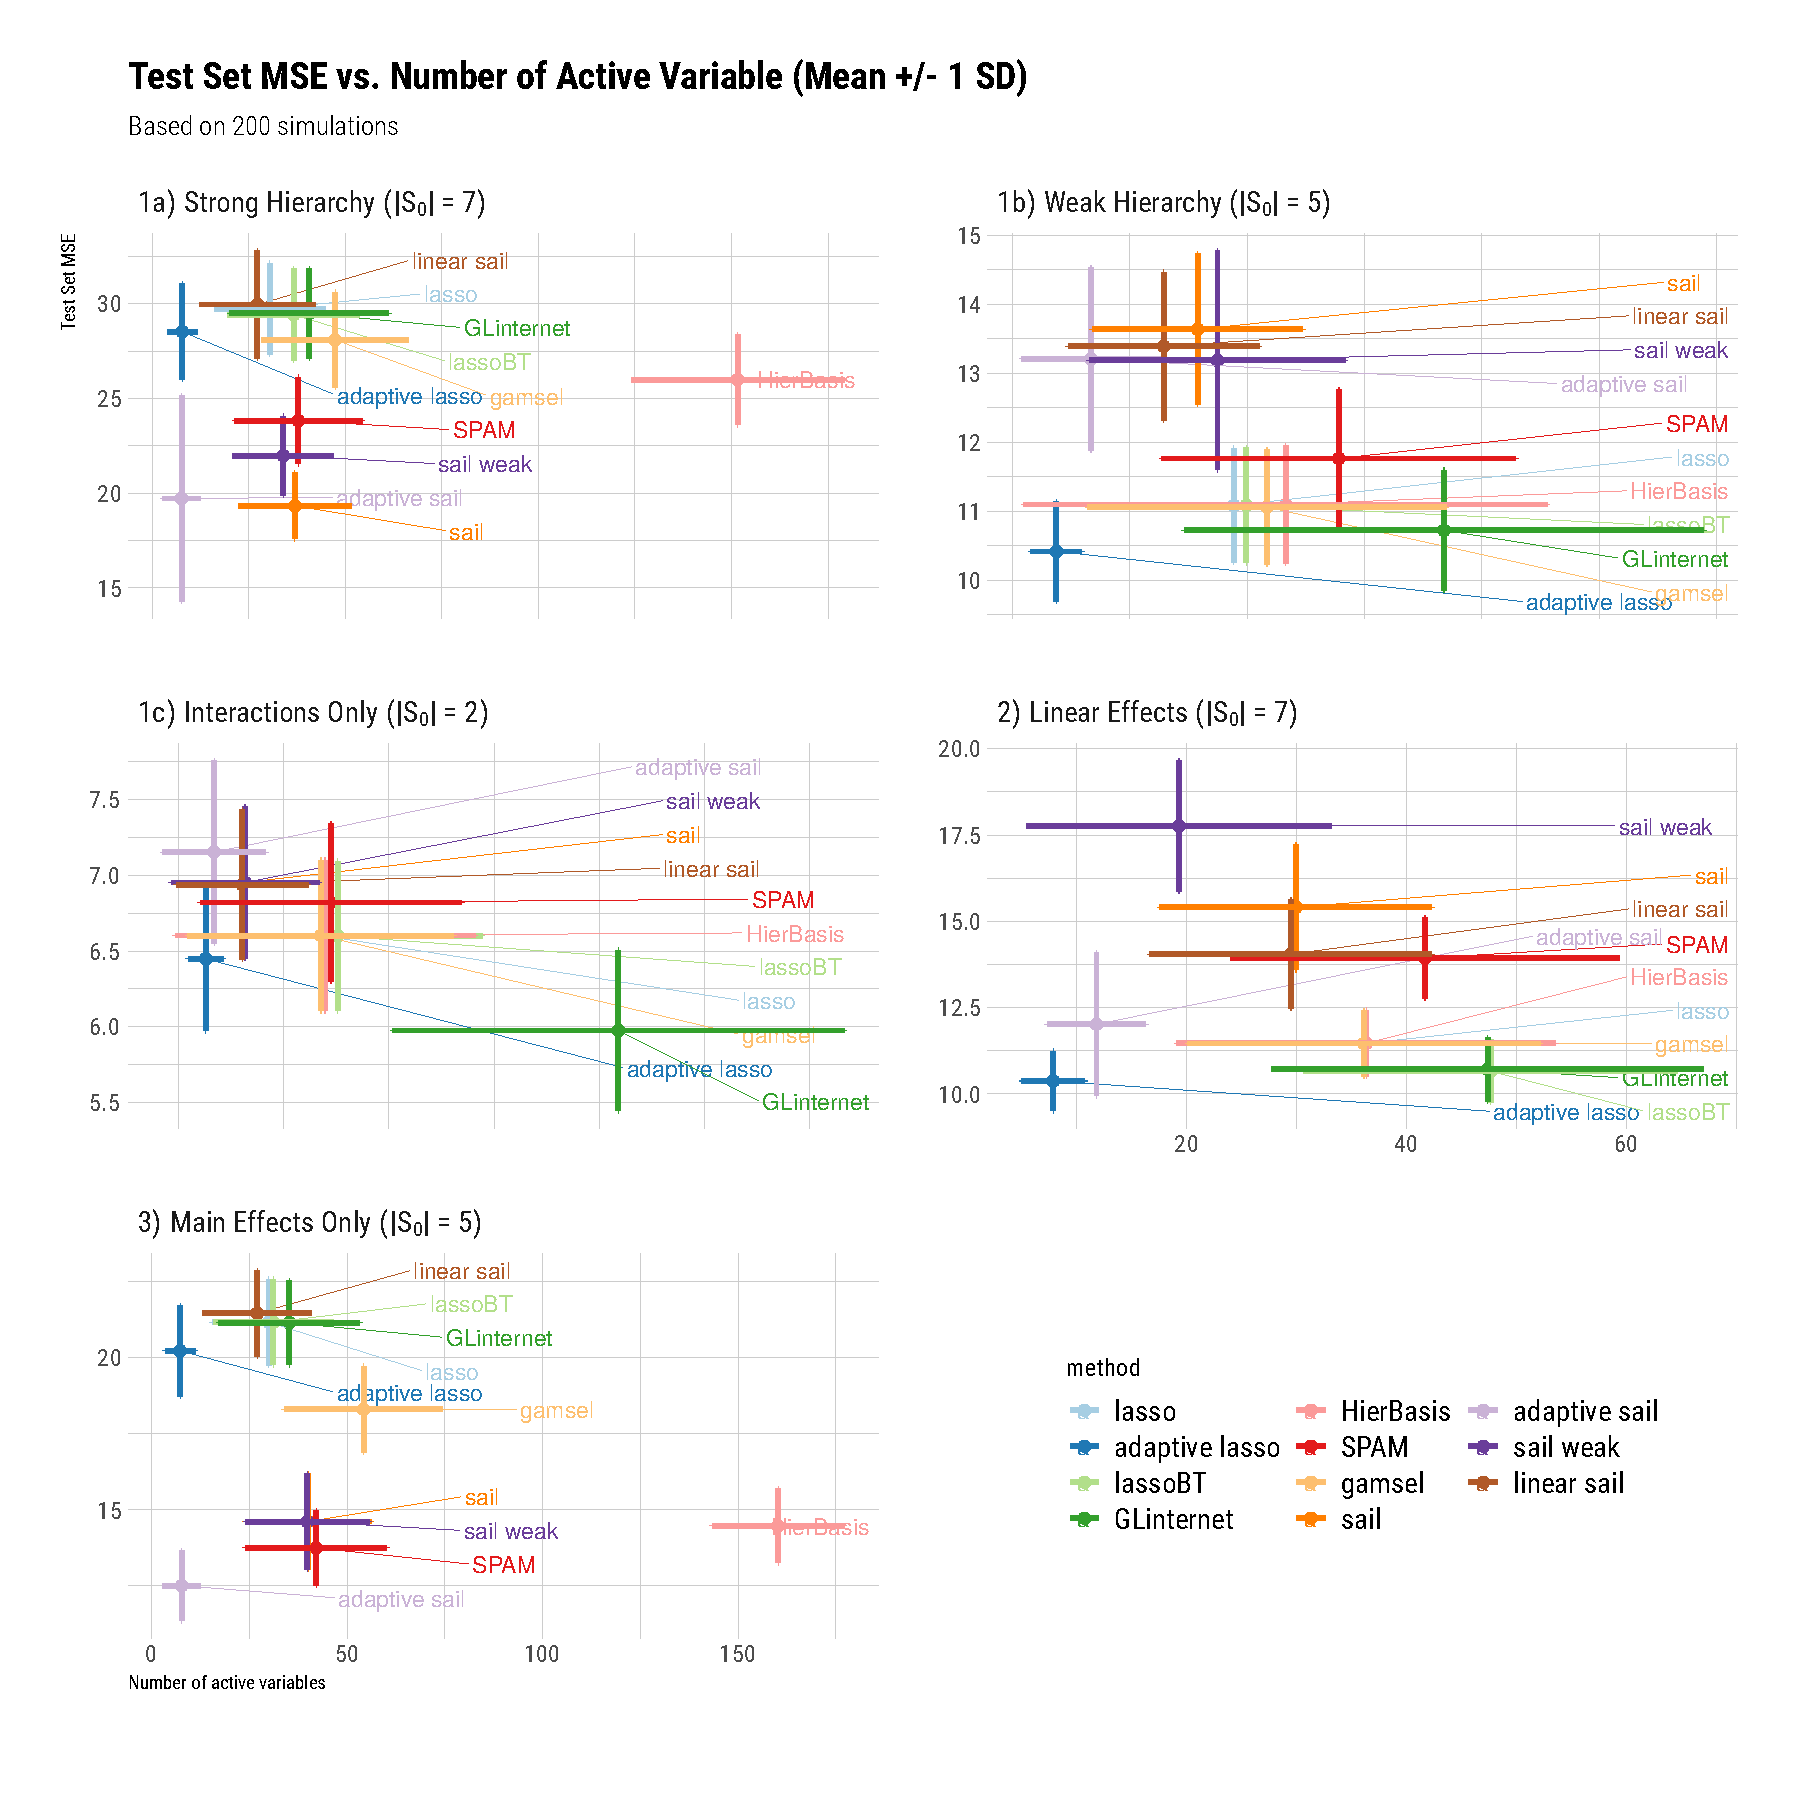
\includegraphics[width=1\linewidth]{figs/plot-mse-nactive-sim-1} 
			
		}
		
		\caption[Test set MSE vs number of active variables results]{Test set MSE vs number of active variables results.}\label{fig:plot-mse-nactive-sim}
	\end{figure}
	
	
\end{knitrout}


\begin{knitrout}\scriptsize
	\definecolor{shadecolor}{rgb}{0.969, 0.969, 0.969}\color{fgcolor}\begin{figure}[H]
		
		{\centering 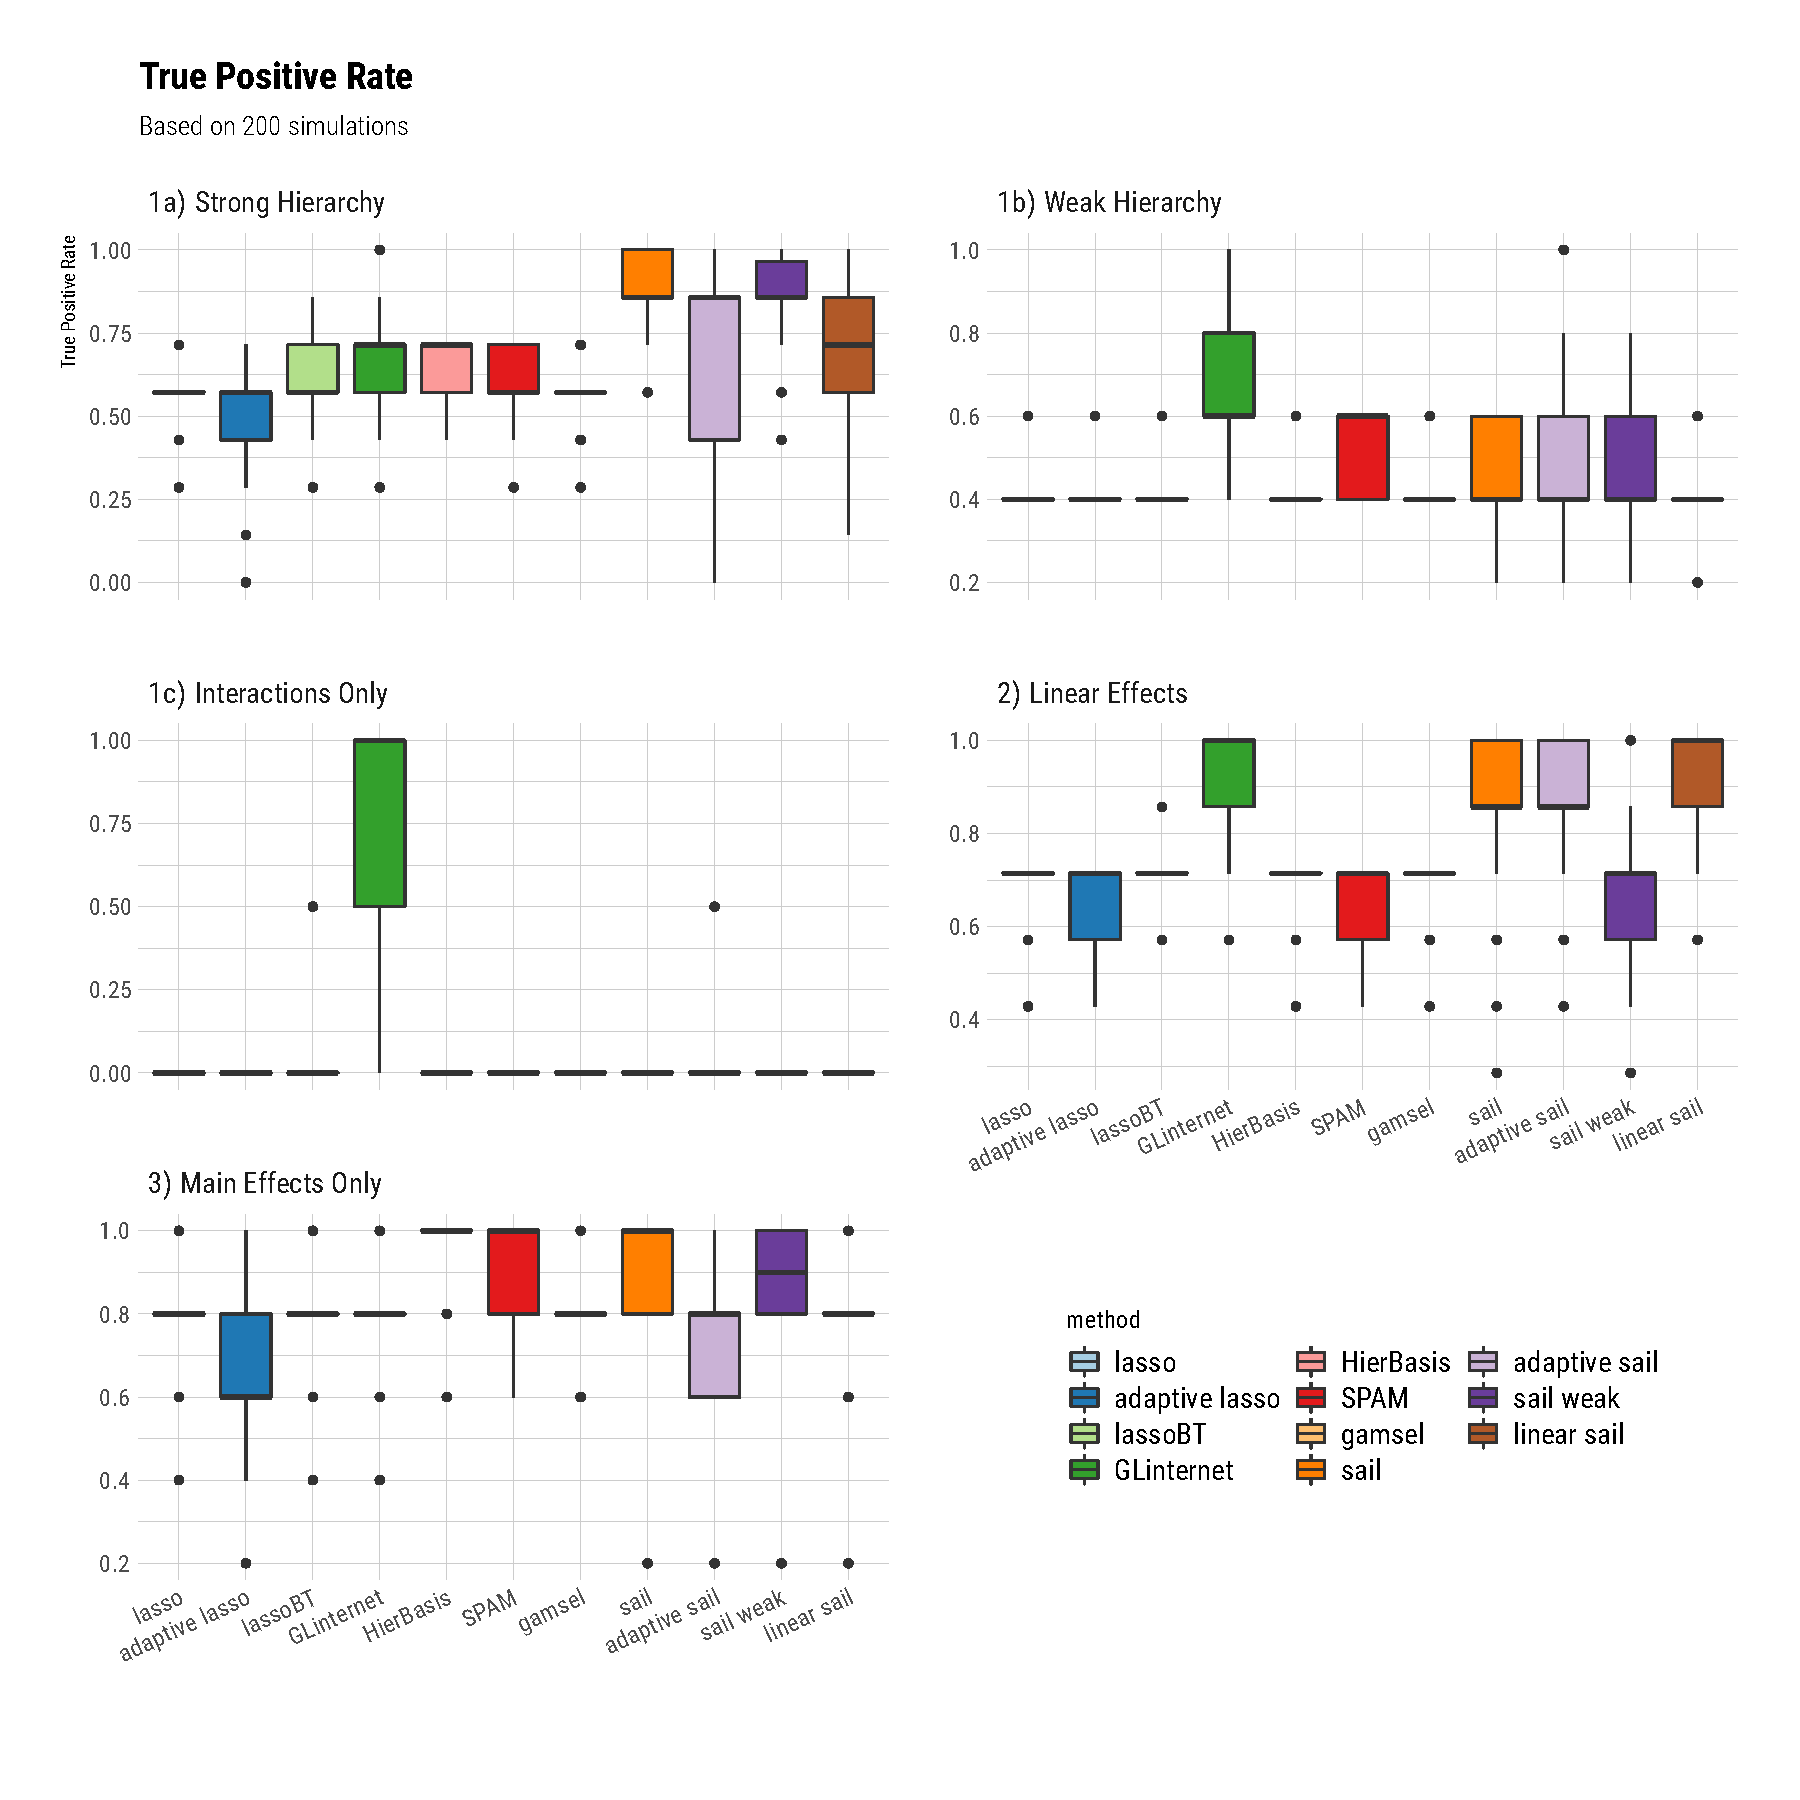
\includegraphics[width=1\linewidth]{figs/plot-tpr-sim-1} 
			
		}
		
		\caption[True positive rate results]{True positive rate results.}\label{fig:plot-tpr-sim}
	\end{figure}
	
	
\end{knitrout}

\begin{knitrout}\scriptsize
	\definecolor{shadecolor}{rgb}{0.969, 0.969, 0.969}\color{fgcolor}\begin{figure}[H]
		
		{\centering 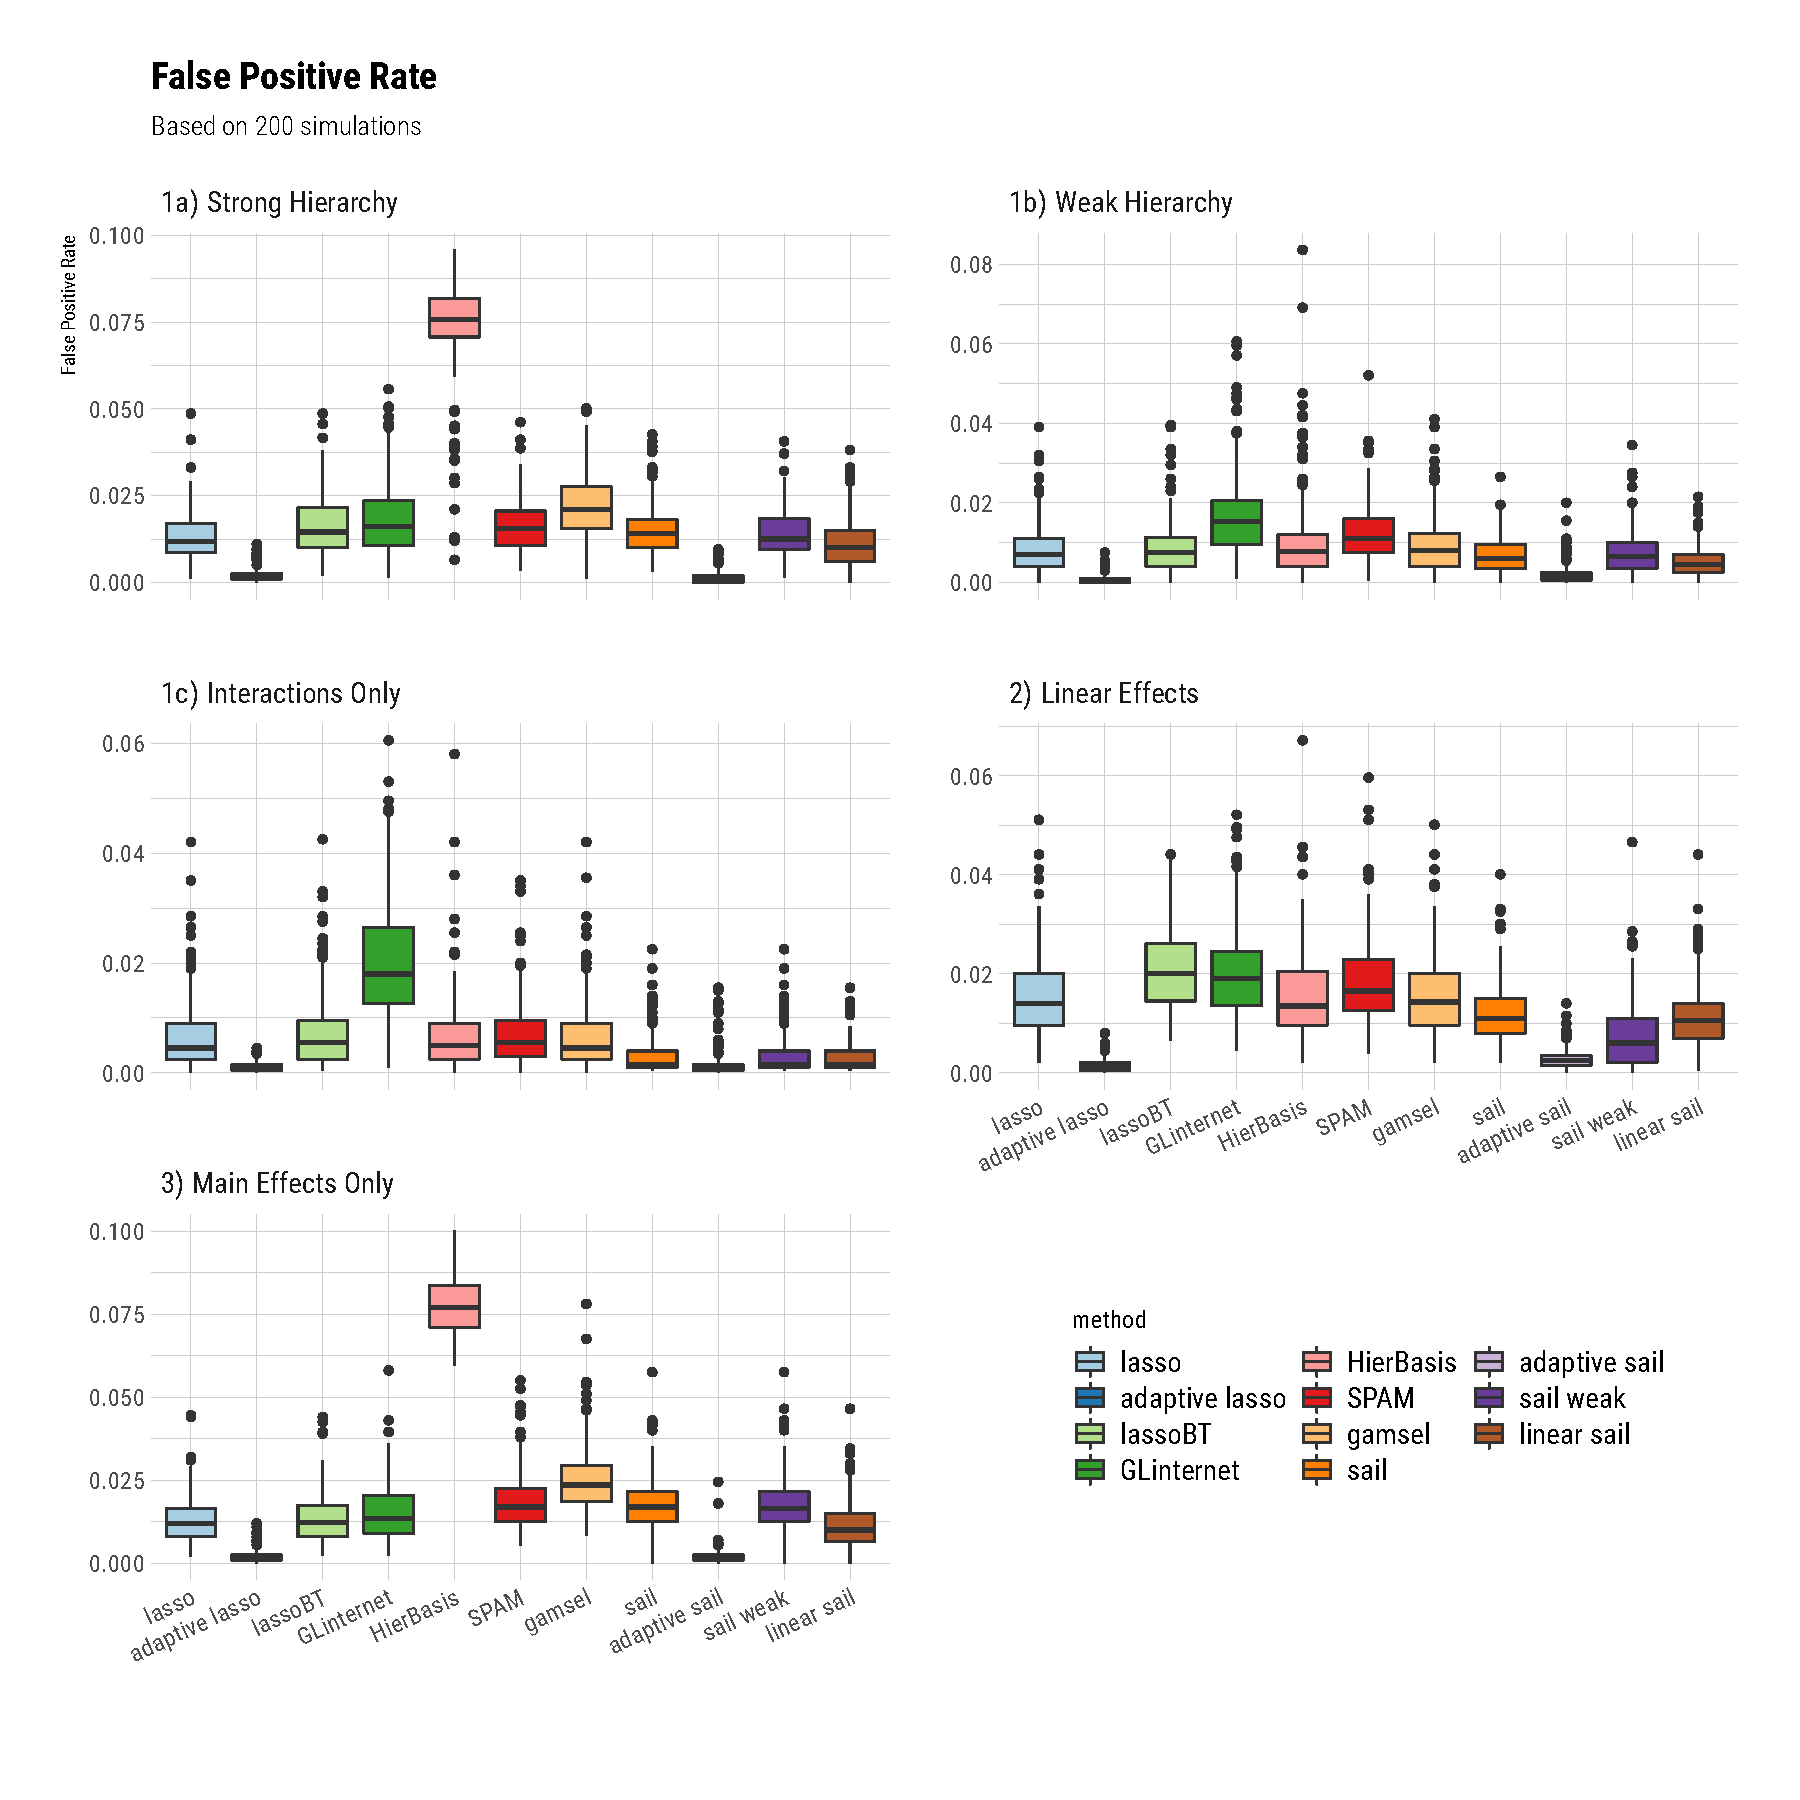
\includegraphics[width=1\linewidth]{figs/plot-fpr-sim-1} 
			
		}
		
		\caption[False positive rate results]{False positive rate results.}\label{fig:plot-fpr-sim}
	\end{figure}
	
	
\end{knitrout}

\begin{knitrout}\scriptsize
	\definecolor{shadecolor}{rgb}{0.969, 0.969, 0.969}\color{fgcolor}\begin{figure}[H]
		
		{\centering 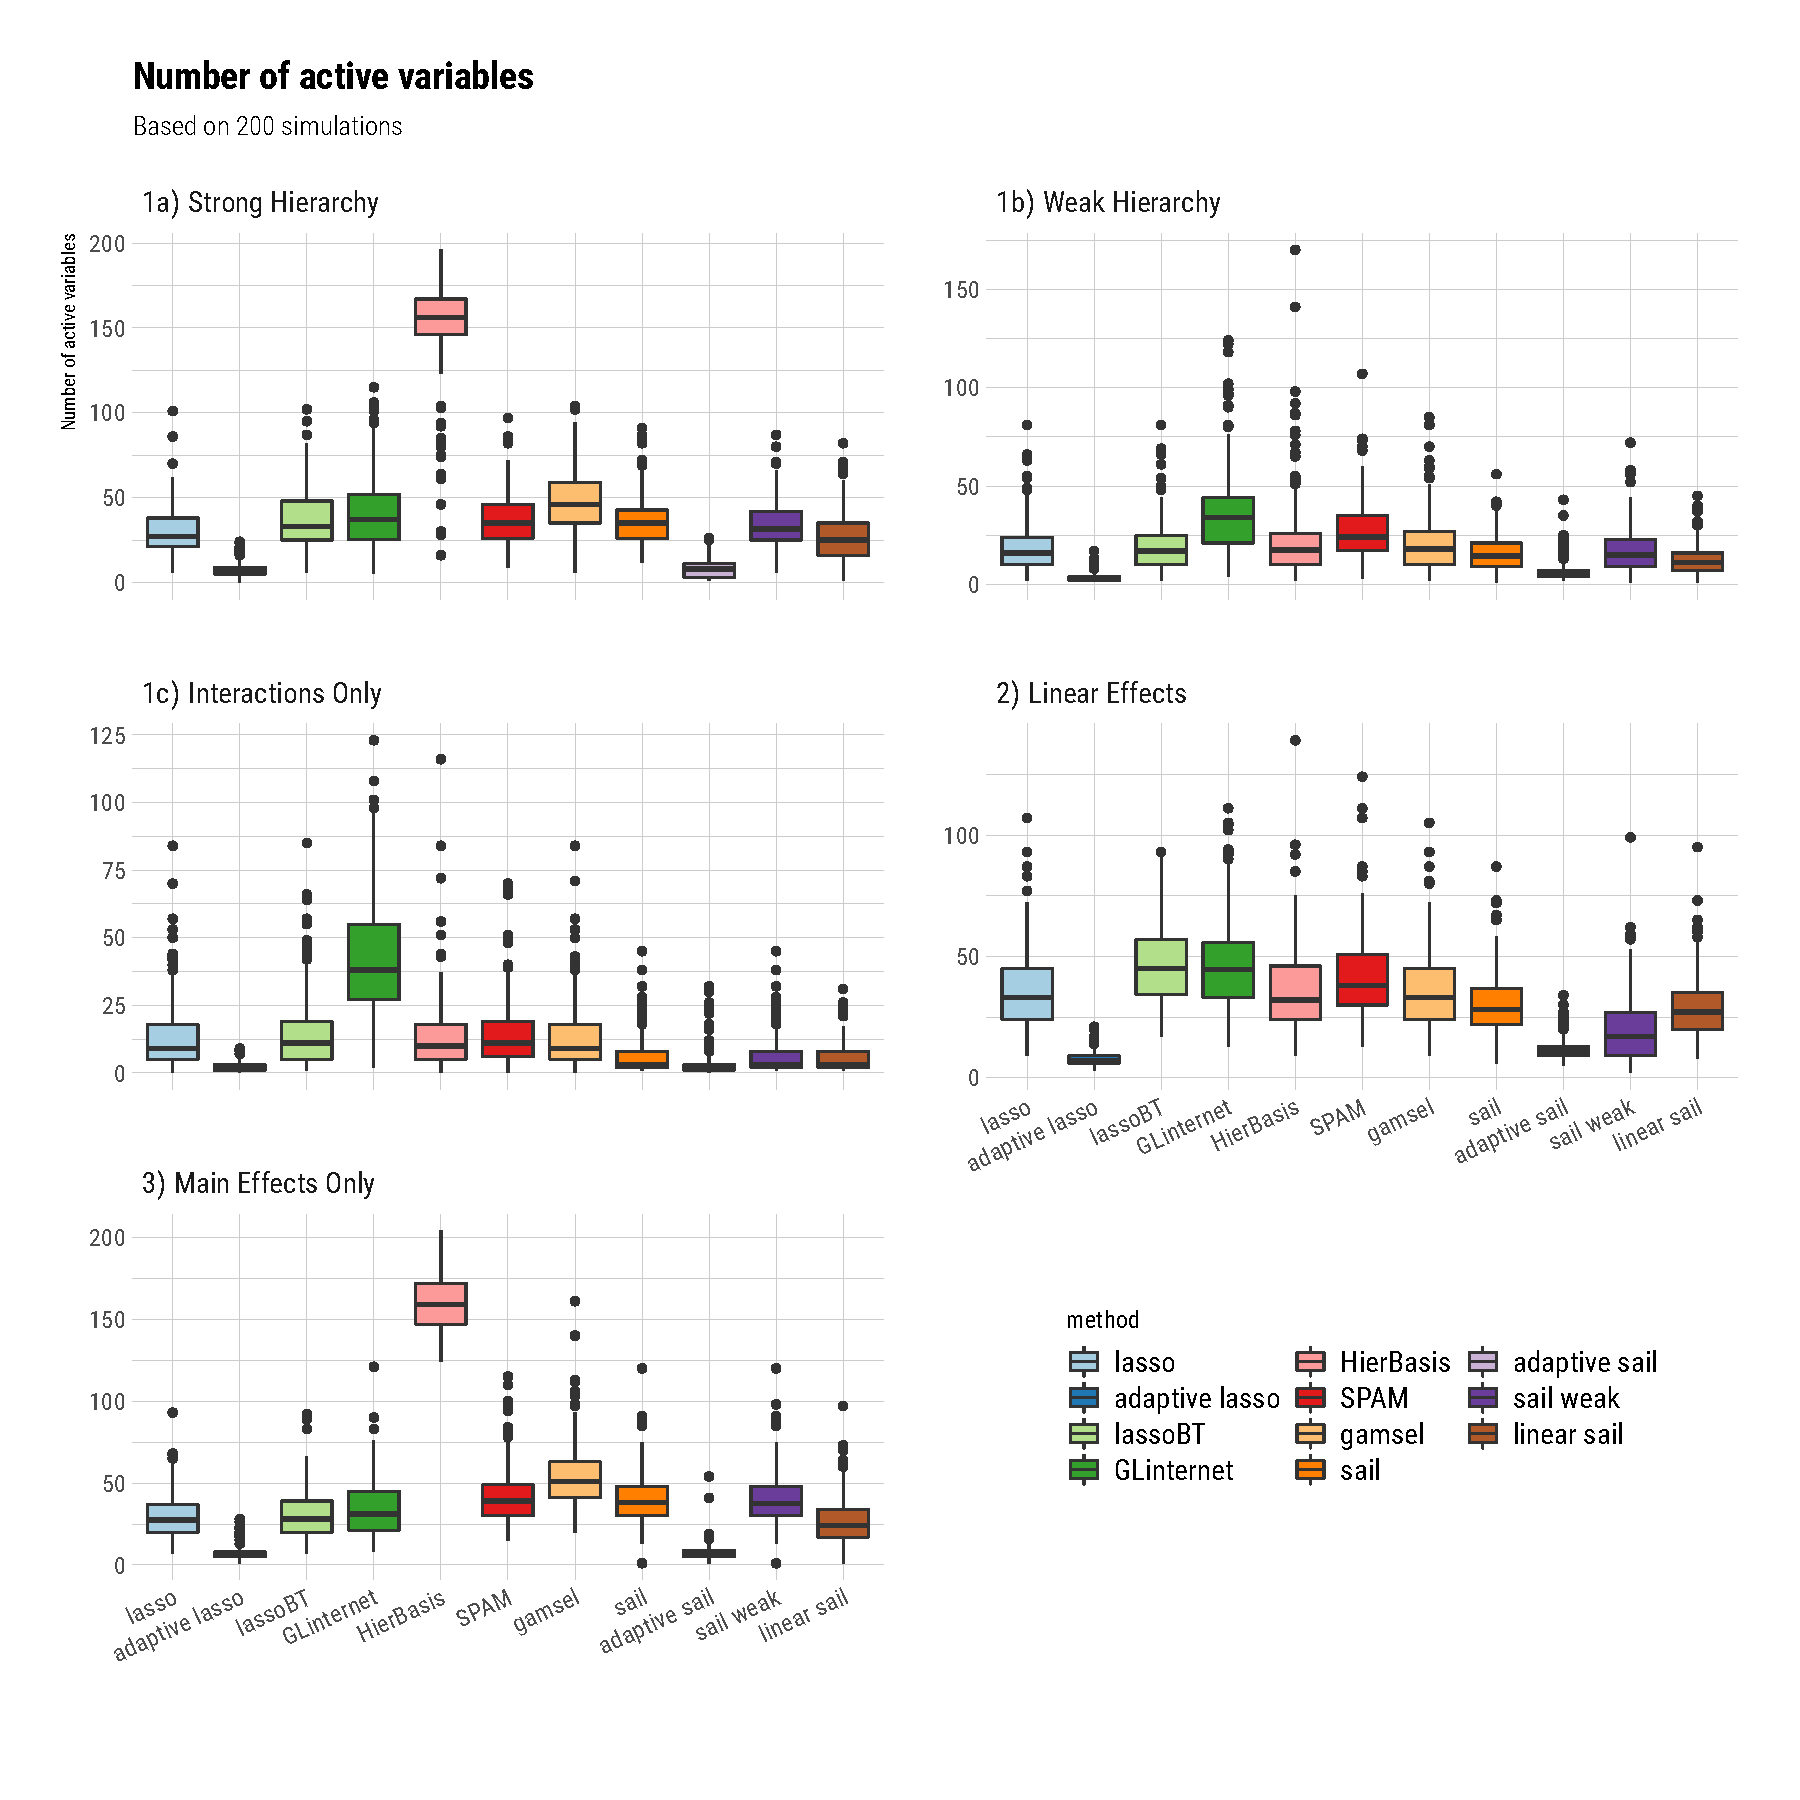
\includegraphics[width=1\linewidth]{figs/plot-nactive-sim-1} 
			
		}
		
		\caption[Number of active variables results]{Number of active variables results.}\label{fig:plot-nactive-sim}
	\end{figure}
	
	
\end{knitrout}


\begin{figure}[H]
	\centering
	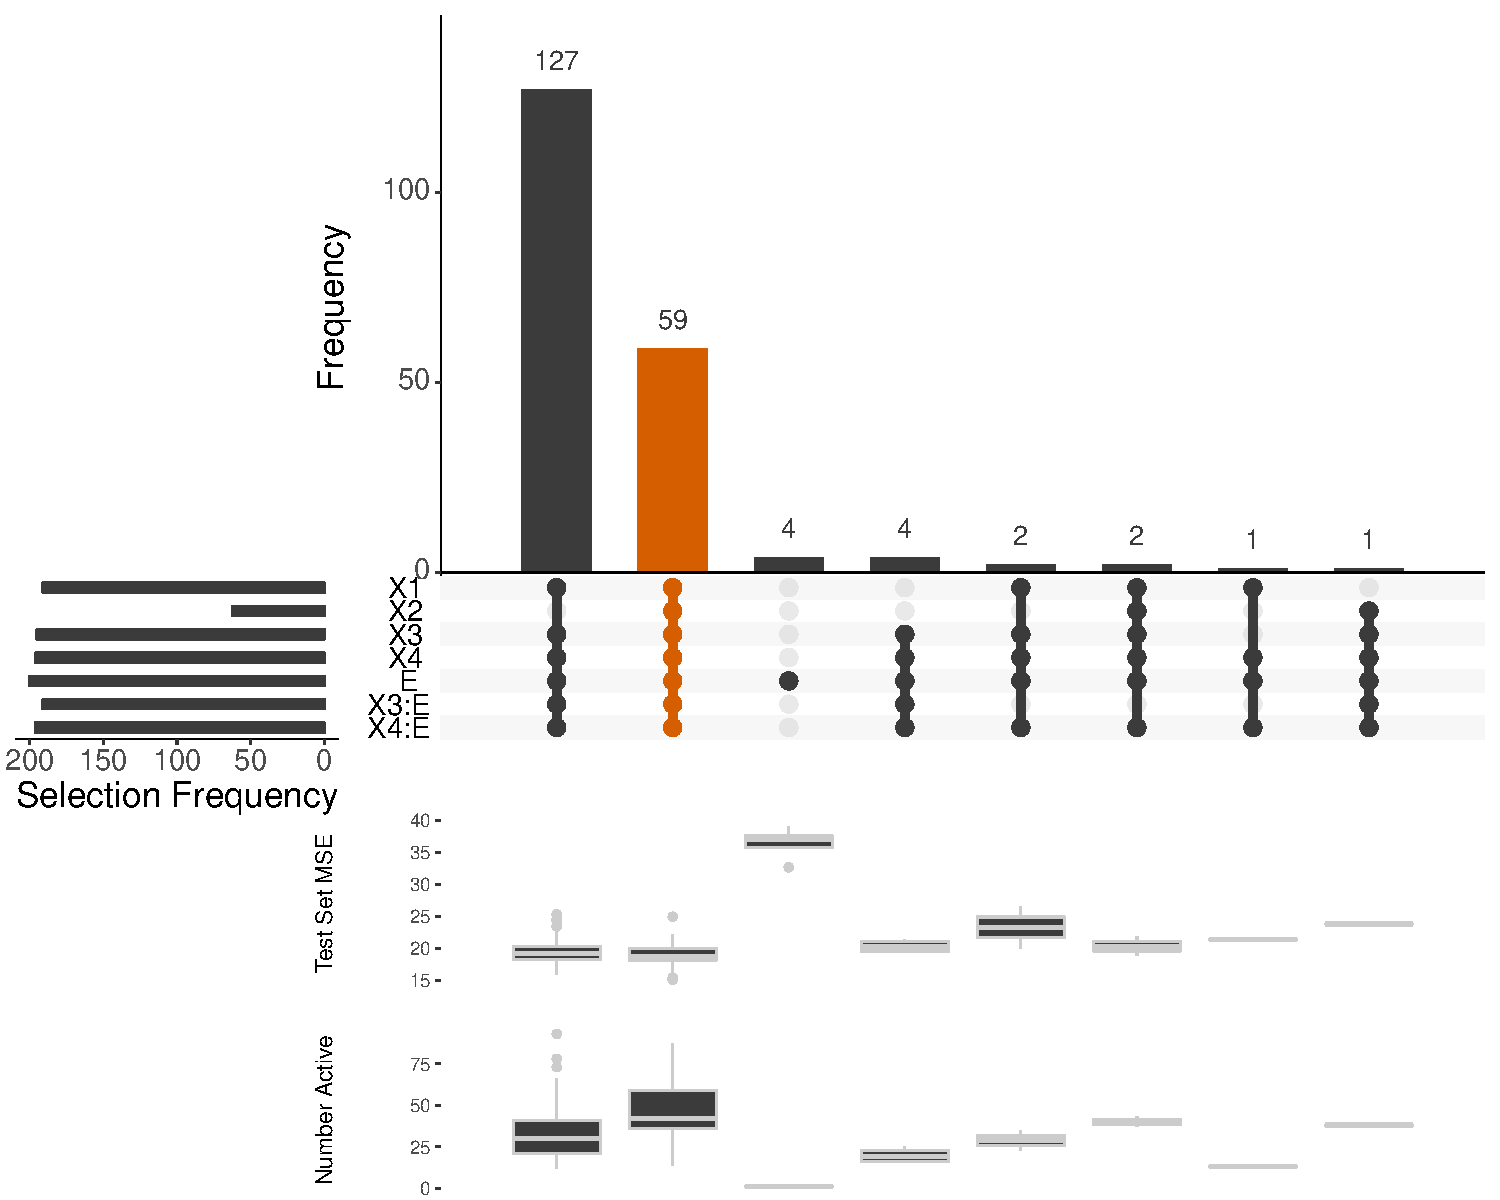
\includegraphics[scale=0.61]{/home/sahir/git_repositories/sail/my_sims/figures/upset_selection_sail_paramIndex1-2-2.pdf}
	\caption{Selection rates across 200 simulations of scenario 1a) for strong heredity \sail.}\label{fig:upset}
\end{figure}

\FloatBarrier 

\section{\sail ~Package Showcase} \label{ap:showcase}

In this section we briefly introduce the freely available and open source \sail ~package in \texttt{R}. More comprehensive documentation is available at \url{https://sahirbhatnagar.com/sail}. Note that this entire section is reproducible; the code and text are combined in an \texttt{.Rnw}\footnote[1]{scripts available at \url{https://github.com/sahirbhatnagar/sail/tree/master/manuscript}} file and compiled using \texttt{knitr}~\citep{xie2015dynamic}. 

\subsection{Installation}

The package can be installed from \href{https://github.com/sahirbhatnagar/sail}{GitHub} via


\begin{knitrout}\scriptsize
	\definecolor{shadecolor}{rgb}{0.969, 0.969, 0.969}\color{fgcolor}\begin{kframe}
		\begin{alltt}
			\hlkwd{install.packages}\hlstd{(}\hlstr{"pacman"}\hlstd{)}
			\hlstd{pacman}\hlopt{::}\hlkwd{p_load_gh}\hlstd{(}\hlstr{'sahirbhatnagar/sail'}\hlstd{)}
		\end{alltt}
	\end{kframe}
\end{knitrout}



\subsection{Quick Start}

We give a quick overview of the main functions and go into details in other vignettes. We will use the simulated data which ships with the package and can be loaded via:

\begin{knitrout}\scriptsize
	\definecolor{shadecolor}{rgb}{0.969, 0.969, 0.969}\color{fgcolor}\begin{kframe}
		\begin{alltt}
			\hlkwd{library}\hlstd{(sail)}
			\hlkwd{data}\hlstd{(}\hlstr{"sailsim"}\hlstd{)}
			\hlkwd{names}\hlstd{(sailsim)}
		\end{alltt}
		\begin{verbatim}
		## [1] "x"        "y"        "e"        "f1"       "f2"       "f3"      
		## [7] "f4"       "f3.inter" "f4.inter"
		\end{verbatim}
	\end{kframe}
\end{knitrout}

We first define a basis expansion. In this example we use B-splines with degree 5.

\begin{knitrout}\scriptsize
	\definecolor{shadecolor}{rgb}{0.969, 0.969, 0.969}\color{fgcolor}\begin{kframe}
		\begin{alltt}
			\hlkwd{library}\hlstd{(splines)}
			\hlstd{f.basis} \hlkwb{<-} \hlkwa{function}\hlstd{(}\hlkwc{x}\hlstd{) splines}\hlopt{::}\hlkwd{bs}\hlstd{(x,} \hlkwc{degree} \hlstd{=} \hlnum{5}\hlstd{)}
		\end{alltt}
	\end{kframe}
\end{knitrout}

Next we fit the model using the most basic call to \sail

\begin{knitrout}\scriptsize
	\definecolor{shadecolor}{rgb}{0.969, 0.969, 0.969}\color{fgcolor}\begin{kframe}
		\begin{alltt}
			\hlstd{fit} \hlkwb{<-} \hlkwd{sail}\hlstd{(}\hlkwc{x} \hlstd{= sailsim}\hlopt{$}\hlstd{x,} \hlkwc{y} \hlstd{= sailsim}\hlopt{$}\hlstd{y,} \hlkwc{e} \hlstd{= sailsim}\hlopt{$}\hlstd{e,} \hlkwc{basis} \hlstd{= f.basis)}
			\end{alltt}
			\end{kframe}
			\end{knitrout}
			
			\texttt{fit} is an object of class \sail ~that contains all the relevant information of the fitted model including the estimated coefficients at each value of $\lambda$ (by default the program chooses its own decreasing sequence of 100 $\lambda$ values). There are \texttt{print}, \texttt{plot}, \texttt{coef} and \texttt{predict} methods of objects of class \sail. 
			
			When \texttt{expand = TRUE} (i.e. the user did not provide their own design matrix), the \texttt{df\_main} and \texttt{df\_interaction} columns correspond to the number of non-zero predictors present in the model before basis expansion. This does not correspond to the number of non-zero coefficients in the model, but rather the number of unique variables. In this example we expanded each column of $\mathbf{X}$ to five columns. If  \texttt{df\_main=4}, \texttt{df\_interaction=2} and \texttt{df\_environment=1}, then the total number of non-zero coefficients would be $5 \times (4+2) + 1$.  
			
			The entire solution path can be plotted via the \texttt{plot} method for objects of class \sail. The y-axis is the value of the coefficient and the x-axis is the $\log(\lambda)$. Each line represents a coefficient in the model, and each color represents a variable (i.e. in this example a given variable will have 5 lines when it is non-zero). The numbers at the top of the plot represent the number of non-zero variables in the model: top panel (\texttt{df\_main} + \texttt{df\_environment}), bottom panel (\texttt{df\_interaction}). The black line is the coefficient path for the environment variable.  
			
			\begin{knitrout}\scriptsize
			\definecolor{shadecolor}{rgb}{0.969, 0.969, 0.969}\color{fgcolor}\begin{kframe}
			\begin{alltt}
			\hlkwd{plot}\hlstd{(fit)}
			\end{alltt}
			\end{kframe}
			
			{\centering 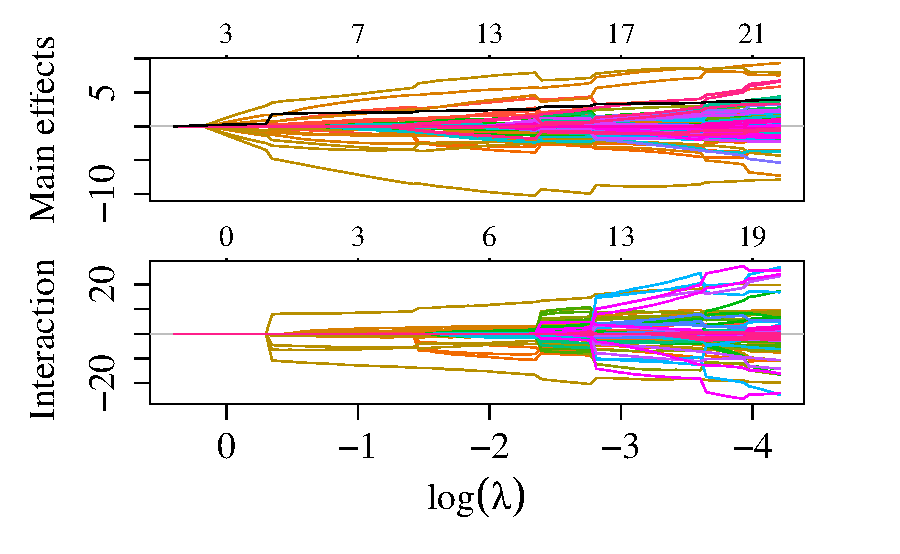
\includegraphics[width=1\linewidth]{figs/sail-solution-path-1} 
				
			}
			
			
			
			\end{knitrout}
			
			
			The estimated coefficients at each value of lambda is given by (matrix partially printed here for brevity)
			
			\begin{knitrout}\scriptsize
			\definecolor{shadecolor}{rgb}{0.969, 0.969, 0.969}\color{fgcolor}\begin{kframe}
			\begin{alltt}
			\hlkwd{coef}\hlstd{(fit)[}\hlnum{1}\hlopt{:}\hlnum{6}\hlstd{,}\hlnum{50}\hlopt{:}\hlnum{55}\hlstd{]}
			\end{alltt}
			\begin{verbatim}
			## 6 x 6 sparse Matrix of class "dgCMatrix"
			##                    s50        s51        s52        s53        s54
			## (Intercept)  5.2908242  5.2837492  5.2803715  5.2753572  5.2717869
			## X1_1        -0.9792849 -0.9604046 -0.9449616 -0.9220738 -0.9171304
			## X1_2         1.6903252  1.7894886  1.8924485  1.9952094  2.1042358
			## X1_3         1.6463057  1.7049842  1.7722916  1.8251613  1.8951562
			## X1_4         1.5224653  1.5433528  1.5663095  1.5854332  1.6102159
			## X1_5         3.3386403  3.4183219  3.4908074  3.5763781  3.6633809
			##                    s55
			## (Intercept)  5.2695399
			## X1_1        -0.9270958
			## X1_2         2.2058453
			## X1_3         1.9642875
			## X1_4         1.6322047
			## X1_5         3.7453708
			\end{verbatim}
			\end{kframe}
			\end{knitrout}
			
			
			
			The corresponding predicted response at each value of lambda (matrix partially printed here for brevity):
			
			\begin{knitrout}\scriptsize
			\definecolor{shadecolor}{rgb}{0.969, 0.969, 0.969}\color{fgcolor}\begin{kframe}
			\begin{alltt}
			\hlkwd{predict}\hlstd{(fit)[}\hlnum{1}\hlopt{:}\hlnum{5}\hlstd{,}\hlnum{50}\hlopt{:}\hlnum{55}\hlstd{]}
			\end{alltt}
			\begin{verbatim}
			##            s50       s51       s52       s53       s54       s55
			## [1,]  6.244693  6.199302  6.185402  6.177991  6.156173  6.124271
			## [2,]  3.002799  2.995418  3.038701  3.079700  3.143715  3.209065
			## [3,]  2.073305  2.043476  2.016319  1.997172  1.966900  1.957271
			## [4,] 13.488945 13.490766 13.360998 13.384370 13.350671 13.324117
			## [5,]  1.225516  1.210346  1.134420  1.156355  1.156696  1.156135
			\end{verbatim}
			\end{kframe}
			\end{knitrout}
			
			
			The predicted response at a specific value of lambda can be specified by the \texttt{s} argument:
			
			\begin{knitrout}\scriptsize
			\definecolor{shadecolor}{rgb}{0.969, 0.969, 0.969}\color{fgcolor}\begin{kframe}
			\begin{alltt}
			\hlkwd{predict}\hlstd{(fit,} \hlkwc{s} \hlstd{=} \hlnum{0.8}\hlstd{)[}\hlnum{1}\hlopt{:}\hlnum{5}\hlstd{, ]}
			\end{alltt}
			\begin{verbatim}
			## [1] 5.624232 4.940944 3.847965 6.687777 3.058125
			\end{verbatim}
			\end{kframe}
			\end{knitrout}
			
			
			You can specify more than one value for `s`:
			
			\begin{knitrout}\scriptsize
			\definecolor{shadecolor}{rgb}{0.969, 0.969, 0.969}\color{fgcolor}\begin{kframe}
			\begin{alltt}
			\hlkwd{predict}\hlstd{(fit,} \hlkwc{s} \hlstd{=} \hlkwd{c}\hlstd{(}\hlnum{0.8}\hlstd{,} \hlnum{0.2}\hlstd{))[}\hlnum{1}\hlopt{:}\hlnum{5}\hlstd{, ]}
			\end{alltt}
			\begin{verbatim}
			##             1         2
			## [1,] 5.624232  6.523025
			## [2,] 4.940944  2.975046
			## [3,] 3.847965  2.326672
			## [4,] 6.687777 13.956092
			## [5,] 3.058125  1.568897
			\end{verbatim}
			\end{kframe}
			\end{knitrout}
			
			
			You can also extract a list of active variables (i.e. variables with a non-zero estimated coefficient) for each value of lambda:
			
			\begin{knitrout}\scriptsize
			\definecolor{shadecolor}{rgb}{0.969, 0.969, 0.969}\color{fgcolor}\begin{kframe}
			\begin{alltt}
			\hlstd{fit[[}\hlstr{"active"}\hlstd{]][}\hlnum{50}\hlopt{:}\hlnum{55}\hlstd{]}
			\end{alltt}
			\begin{verbatim}
			## [[1]]
			##  [1] "X1"    "X2"    "X3"    "X4"    "X8"    "X10"   "X11"   "X20"  
			##  [9] "X1:E"  "X2:E"  "X3:E"  "X4:E"  "X8:E"  "X11:E" "E"    
			## 
			## [[2]]
			##  [1] "X1"    "X2"    "X3"    "X4"    "X6"    "X8"    "X10"   "X11"  
			##  [9] "X20"   "X1:E"  "X2:E"  "X3:E"  "X4:E"  "X8:E"  "X11:E" "E"    
			## 
			## [[3]]
			##  [1] "X1"    "X2"    "X3"    "X4"    "X6"    "X8"    "X10"   "X11"  
			##  [9] "X16"   "X20"   "X1:E"  "X2:E"  "X3:E"  "X4:E"  "X8:E"  "X11:E"
			## [17] "E"    
			## 
			## [[4]]
			##  [1] "X1"    "X2"    "X3"    "X4"    "X6"    "X8"    "X10"   "X11"  
			##  [9] "X15"   "X16"   "X19"   "X20"   "X1:E"  "X2:E"  "X3:E"  "X4:E" 
			## [17] "X8:E"  "X11:E" "E"    
			## 
			## [[5]]
			##  [1] "X1"    "X2"    "X3"    "X4"    "X5"    "X6"    "X8"    "X10"  
			##  [9] "X11"   "X15"   "X16"   "X19"   "X20"   "X1:E"  "X2:E"  "X3:E" 
			## [17] "X4:E"  "X8:E"  "X11:E" "E"    
			## 
			## [[6]]
			##  [1] "X1"    "X2"    "X3"    "X4"    "X5"    "X6"    "X8"    "X10"  
			##  [9] "X11"   "X15"   "X16"   "X19"   "X20"   "X1:E"  "X2:E"  "X3:E" 
			## [17] "X4:E"  "X8:E"  "X11:E" "E"
			\end{verbatim}
			\end{kframe}
			\end{knitrout}
			
			
			\subsection{Cross-Validation}
			
			\texttt{cv.sail} is the main function to do cross-validation along with \texttt{plot}, \texttt{predict}, and \texttt{coef} methods for objects of class \texttt{cv.sail}. We run it in parallel:
			
			\begin{knitrout}\scriptsize
			\definecolor{shadecolor}{rgb}{0.969, 0.969, 0.969}\color{fgcolor}\begin{kframe}
			\begin{alltt}
			\hlkwd{set.seed}\hlstd{(}\hlnum{432}\hlstd{)} \hlcom{# to reproduce results (randomness due to CV folds)}
			\hlkwd{library}\hlstd{(doMC)}
			\hlkwd{registerDoMC}\hlstd{(}\hlkwc{cores} \hlstd{=} \hlnum{8}\hlstd{)}
			\hlstd{cvfit} \hlkwb{<-} \hlkwd{cv.sail}\hlstd{(}\hlkwc{x} \hlstd{= sailsim}\hlopt{$}\hlstd{x,} \hlkwc{y} \hlstd{= sailsim}\hlopt{$}\hlstd{y,} \hlkwc{e} \hlstd{= sailsim}\hlopt{$}\hlstd{e,} \hlkwc{basis} \hlstd{= f.basis,}
			\hlkwc{nfolds} \hlstd{=} \hlnum{5}\hlstd{,} \hlkwc{parallel} \hlstd{=} \hlnum{TRUE}\hlstd{)}
		\end{alltt}
	\end{kframe}
\end{knitrout}

We plot the cross-validated error curve which has the mean-squared error on the y-axis and $\log(\lambda)$ on the x-axis. It includes the cross-validation curve (red dotted line), and upper and lower standard deviation curves along the $\lambda$ sequence (error bars). Two selected $\lambda$'s are indicated by the vertical dotted lines (see below). The numbers at the top of the plot represent the total number of non-zero variables at that value of $\lambda$ (\texttt{df\_main} + \texttt{df\_environment} + \texttt{df\_interaction}):


\begin{knitrout}\scriptsize
	\definecolor{shadecolor}{rgb}{0.969, 0.969, 0.969}\color{fgcolor}\begin{kframe}
		\begin{alltt}
			\hlkwd{plot}\hlstd{(cvfit)}
		\end{alltt}
	\end{kframe}
	
	{\centering 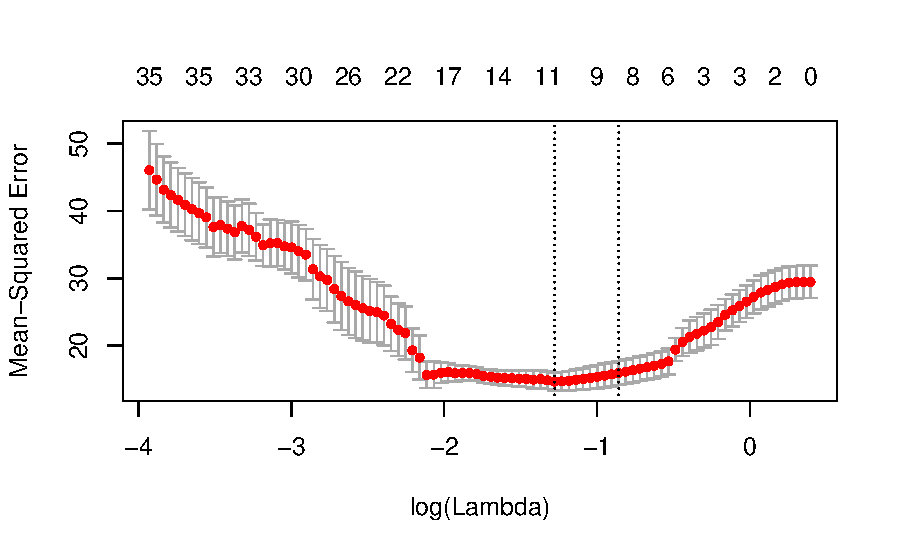
\includegraphics[width=1\linewidth]{figs/sail-cv-1} 
		
	}
	
	
	
\end{knitrout}

\texttt{lambda.min} is the value of $\lambda$ that gives minimum mean cross-validated error. The other $\lambda$ saved is \texttt{lambda.1se},
which gives the most regularized model such that error is within one standard error of the minimum. We can view the selected $\lambda$'s and the corresponding coefficients:

\begin{knitrout}\scriptsize
	\definecolor{shadecolor}{rgb}{0.969, 0.969, 0.969}\color{fgcolor}\begin{kframe}
		\begin{alltt}
			\hlstd{cvfit[[}\hlstr{"lambda.min"}\hlstd{]]}
		\end{alltt}
		\begin{verbatim}
		## [1] 0.2788355
		\end{verbatim}
		\begin{alltt}
			\hlstd{cvfit[[}\hlstr{"lambda.1se"}\hlstd{]]}
		\end{alltt}
		\begin{verbatim}
		## [1] 0.4238052
		\end{verbatim}
	\end{kframe}
\end{knitrout}

The estimated nonzero coefficients at \texttt{lambda.1se} and \texttt{lambda.min}:

\begin{knitrout}\scriptsize
	\definecolor{shadecolor}{rgb}{0.969, 0.969, 0.969}\color{fgcolor}\begin{kframe}
		\begin{alltt}
			\hlkwd{predict}\hlstd{(cvfit,} \hlkwc{type} \hlstd{=} \hlstr{"nonzero"}\hlstd{,} \hlkwc{s}\hlstd{=}\hlstr{"lambda.1se"}\hlstd{)} \hlcom{# lambda.1se is the default}
		\end{alltt}
		\begin{verbatim}
		##                        1
		## (Intercept)   5.42162330
		## X1_1         -0.78259292
		## X1_2          0.13434743
		## X1_3          0.43872182
		## X1_4          0.79452833
		## X1_5          1.92193021
		## X3_1          3.45123833
		## X3_2          1.56772288
		## X3_3         -1.27179135
		## X3_4         -2.27792209
		## X3_5         -1.23352137
		## X4_1          4.47182924
		## X4_2         -2.87488058
		## X4_3         -6.65073351
		## X4_4         -3.44085202
		## X4_5         -0.47032703
		## X8_1          0.17507051
		## X8_2          0.11619435
		## X8_3          0.01783624
		## X8_4         -0.10505726
		## X8_5         -0.24485431
		## X11_1         0.13691003
		## X11_2         0.02857999
		## X11_3        -0.07324928
		## X11_4        -0.20944262
		## X11_5        -0.22648392
		## E             1.99575642
		## X3_1:E        1.80711590
		## X3_2:E        0.82088128
		## X3_3:E       -0.66592746
		## X3_4:E       -1.19275137
		## X3_5:E       -0.64588877
		## X4_1:E        8.31249627
		## X4_2:E       -5.34399523
		## X4_3:E      -12.36277025
		## X4_4:E       -6.39605585
		## X4_5:E       -0.87427125
		\end{verbatim}
		\begin{alltt}
			\hlkwd{predict}\hlstd{(cvfit,} \hlkwc{type} \hlstd{=} \hlstr{"nonzero"}\hlstd{,} \hlkwc{s} \hlstd{=} \hlstr{"lambda.min"}\hlstd{)}
		\end{alltt}
		\begin{verbatim}
		##                        1
		## (Intercept)   5.43619834
		## X1_1         -1.23832799
		## X1_2          0.48736979
		## X1_3          0.88915804
		## X1_4          1.10813495
		## X1_5          2.68123247
		## X2_1         -0.21985179
		## X2_2         -0.95071069
		## X2_3         -0.76066212
		## X2_4         -0.17413616
		## X2_5         -0.06845895
		## X3_1          4.42751615
		## X3_2          2.28700197
		## X3_3         -1.36817303
		## X3_4         -2.56642377
		## X3_5         -1.03093978
		## X4_1          5.37962120
		## X4_2         -3.35568118
		## X4_3         -8.07355346
		## X4_4         -3.50305791
		## X4_5         -0.55031385
		## X8_1          0.47925233
		## X8_2          0.33992532
		## X8_3          0.07652614
		## X8_4         -0.28114406
		## X8_5         -0.66616044
		## X11_1         0.34768804
		## X11_2         0.06274138
		## X11_3        -0.20149241
		## X11_4        -0.67859653
		## X11_5        -0.69589312
		## X20_1         0.10225010
		## X20_2        -0.03831915
		## X20_3        -0.17781683
		## X20_4        -0.18564133
		## X20_5         0.09741855
		## E             2.06410796
		## X1_1:E       -0.53459297
		## X1_2:E        0.21040020
		## X1_3:E        0.38385439
		## X1_4:E        0.47838792
		## X1_5:E        1.15750273
		## X3_1:E        2.37995847
		## X3_2:E        1.22935061
		## X3_3:E       -0.73544508
		## X3_4:E       -1.37955047
		## X3_5:E       -0.55416937
		## X4_1:E        8.87349228
		## X4_2:E       -5.53507578
		## X4_3:E      -13.31703694
		## X4_4:E       -5.77816841
		## X4_5:E       -0.90772296
		\end{verbatim}
	\end{kframe}
\end{knitrout}



\subsection{Visualizing the Effect of the Non-linear Terms}

B-splines are difficult to interpret. We provide a plotting function to visualize the effect of the non-linear function on the response.

\subsubsection{Main Effects}

Since we are using simulated data, we also plot the true curve:

\begin{knitrout}\scriptsize
	\definecolor{shadecolor}{rgb}{0.969, 0.969, 0.969}\color{fgcolor}\begin{kframe}
		\begin{alltt}
			\hlkwd{plotMain}\hlstd{(cvfit}\hlopt{$}\hlstd{sail.fit,} \hlkwc{x} \hlstd{= sailsim}\hlopt{$}\hlstd{x,} \hlkwc{xvar} \hlstd{=} \hlstr{"X3"}\hlstd{,}
			\hlkwc{legend.position} \hlstd{=} \hlstr{"topright"}\hlstd{,}
			\hlkwc{s} \hlstd{= cvfit}\hlopt{$}\hlstd{lambda.min,} \hlkwc{f.truth} \hlstd{= sailsim}\hlopt{$}\hlstd{f3)}
		\end{alltt}
	\end{kframe}
	
	{\centering 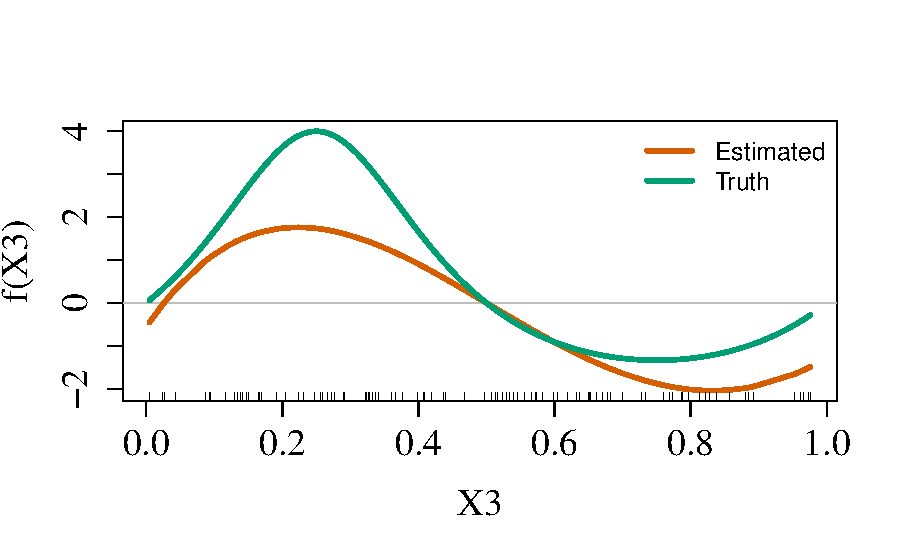
\includegraphics[width=1\linewidth]{figs/sail-main-eff-1} 
		
	}
	
	
	
\end{knitrout}


\subsubsection{Interaction Effects}

Again, since we are using simulated data, we also plot the true interaction:

\begin{knitrout}\scriptsize
	\definecolor{shadecolor}{rgb}{0.969, 0.969, 0.969}\color{fgcolor}\begin{kframe}
		\begin{alltt}
			\hlkwd{plotInter}\hlstd{(cvfit}\hlopt{$}\hlstd{sail.fit,} \hlkwc{x} \hlstd{= sailsim}\hlopt{$}\hlstd{x,} \hlkwc{xvar} \hlstd{=} \hlstr{"X4"}\hlstd{,}
			\hlkwc{f.truth} \hlstd{= sailsim}\hlopt{$}\hlstd{f4.inter,}
			\hlkwc{s} \hlstd{= cvfit}\hlopt{$}\hlstd{lambda.min,}
			\hlkwc{title_z} \hlstd{=} \hlstr{"Estimated"}\hlstd{)}
		\end{alltt}
	\end{kframe}
	
	{\centering 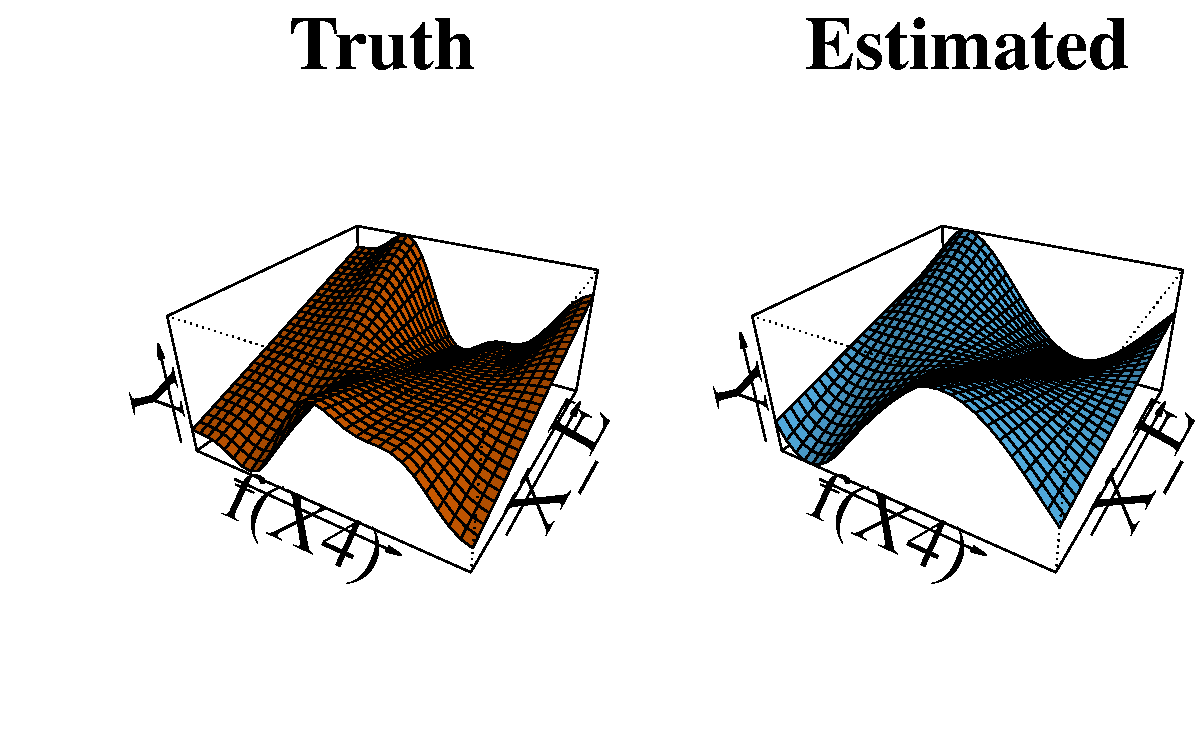
\includegraphics[width=1\linewidth]{figs/sail-inter-eff-1} 
		
	}
	
	
	
\end{knitrout}



\subsection{Linear Interactions}

The \texttt{basis} argument in the \texttt{sail} function is very flexible in that it allows you to apply \textit{any} basis expansion to the columns of $\mathbf{X}$. Of course, there might be situations where you do not expect any non-linear main effects or interactions to be present in your data. You can still use the \sail ~method to search for linear main effects and interactions. This can be accomplished by specifying an identity map:

\begin{knitrout}\scriptsize
	\definecolor{shadecolor}{rgb}{0.969, 0.969, 0.969}\color{fgcolor}\begin{kframe}
		\begin{alltt}
			\hlstd{f.identity} \hlkwb{<-} \hlkwa{function}\hlstd{(}\hlkwc{i}\hlstd{) i}
		\end{alltt}
	\end{kframe}
\end{knitrout}

We then pass this function to the \texttt{basis} argument in \texttt{cv.sail}:

\begin{knitrout}\scriptsize
	\definecolor{shadecolor}{rgb}{0.969, 0.969, 0.969}\color{fgcolor}\begin{kframe}
		\begin{alltt}
			\hlstd{cvfit_linear} \hlkwb{<-} \hlkwd{cv.sail}\hlstd{(}\hlkwc{x} \hlstd{= sailsim}\hlopt{$}\hlstd{x,} \hlkwc{y} \hlstd{= sailsim}\hlopt{$}\hlstd{y,} \hlkwc{e} \hlstd{= sailsim}\hlopt{$}\hlstd{e,}
			\hlkwc{basis} \hlstd{= f.identity,} \hlkwc{nfolds} \hlstd{=} \hlnum{5}\hlstd{,} \hlkwc{parallel} \hlstd{=} \hlnum{TRUE}\hlstd{)}
			\end{alltt}
			\end{kframe}
			\end{knitrout}
			
			
			Next we plot the cross-validated curve:
			
			\begin{knitrout}\scriptsize
			\definecolor{shadecolor}{rgb}{0.969, 0.969, 0.969}\color{fgcolor}\begin{kframe}
			\begin{alltt}
			\hlkwd{plot}\hlstd{(cvfit_linear)}
			\end{alltt}
			\end{kframe}
			
			{\centering 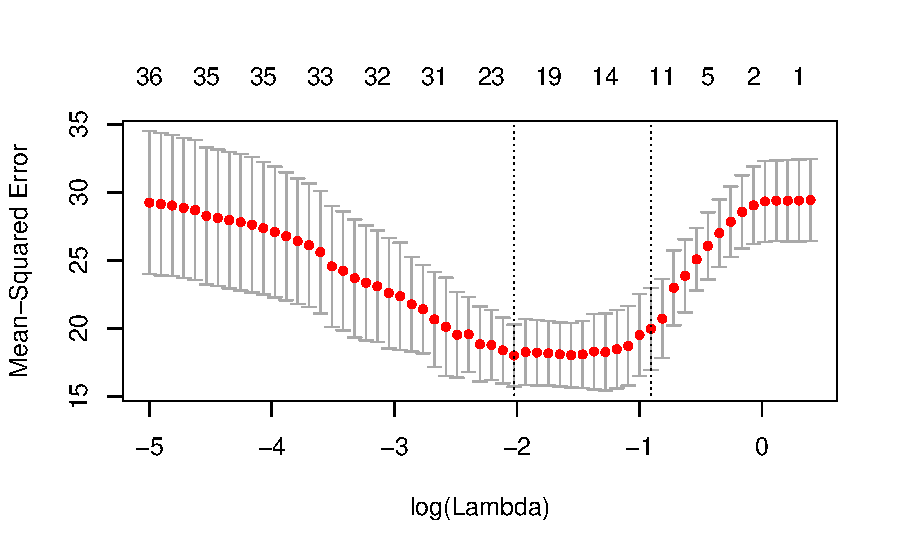
\includegraphics[width=1\linewidth]{figs/sail-solution-path-linear-1} 
				
			}
			
			
			
			\end{knitrout}
			
			And extract the model at \texttt{lambda.min}:
			
			\begin{knitrout}\scriptsize
			\definecolor{shadecolor}{rgb}{0.969, 0.969, 0.969}\color{fgcolor}\begin{kframe}
			\begin{alltt}
			\hlkwd{predict}\hlstd{(cvfit_linear,} \hlkwc{s} \hlstd{=} \hlstr{"lambda.min"}\hlstd{,} \hlkwc{type} \hlstd{=} \hlstr{"nonzero"}\hlstd{)}
			\end{alltt}
			\begin{verbatim}
			##                       1
			## (Intercept)   5.4385240
			## X1_1          2.4568930
			## X2_1         -1.6517024
			## X3_1         -5.1516226
			## X4_1         -7.1356296
			## X7_1         -1.1055458
			## X8_1         -0.8602620
			## X11_1        -2.1990021
			## X14_1        -1.9208459
			## X16_1         3.2004798
			## X18_1         1.0234994
			## X20_1        -0.2161983
			## E             2.4466403
			## X1_1:E       -4.3995787
			## X2_1:E       -2.7115733
			## X3_1:E       -4.7198552
			## X4_1:E      -12.9777976
			## X7_1:E        2.3705634
			## X11_1:E      -2.1462985
			## X14_1:E      -0.9788318
			## X16_1:E       6.9268058
			## X18_1:E       1.9005742
			\end{verbatim}
			\end{kframe}
			\end{knitrout}
			
			
			\subsection{Applying a different penalty to each predictor} \label{ap:pfac}
			
			Recall that we consider the following penalized least squares criterion for this problem:
			
			\begin{equation}
			\arg\min_{\boldsymbol{\theta} }  \mathcal{L}(Y;\boldsymbol{\theta}) + \lambda (1-\alpha)  \left( w_E |\beta_E| + \sum_{j=1}^{p} w_j \lVert\boldsymbol{\theta}_j \rVert_2 \right) +  \lambda\alpha \sum_{j=1}^{p} w_{jE} |\gamma_{j}| 
			\end{equation} 
			
			The weights $w_E, w_j, w_{jE}$ are by default set to 1 as specified by the \texttt{penalty.factor} argument. This argument allows users to apply separate penalty factors to each coefficient.  In particular, any variable with \texttt{penalty.factor} equal to zero is not penalized at all. This feature can be applied mainly for two reasons:  
			
			1. Prior knowledge about the importance of certain variables is known. Larger weights will penalize the variable more, while smaller weights will penalize the variable less  
			2. Allows users to apply the Adaptive \sail, ~similar to the \href{http://users.stat.umn.edu/~zouxx019/Papers/adalasso.pdf}{Adaptive Lasso}  
			
			In the following example, we want the environment variable to always be included so we set the first element of \texttt{p.fac} to zero. We also want to apply less of a penalty to the main effects for $X_2, X_3, X_4$:
			
			\begin{knitrout}\scriptsize
			\definecolor{shadecolor}{rgb}{0.969, 0.969, 0.969}\color{fgcolor}\begin{kframe}
			\begin{alltt}
			\hlcom{# the weights correspond to E, X1, X2, X3, ... X_p, X1:E, X2:E, ... X_p:E}
			\hlstd{p.fac} \hlkwb{<-} \hlkwd{c}\hlstd{(}\hlnum{0}\hlstd{,} \hlnum{1}\hlstd{,} \hlnum{0.4}\hlstd{,} \hlnum{0.6}\hlstd{,} \hlnum{0.7}\hlstd{,} \hlkwd{rep}\hlstd{(}\hlnum{1}\hlstd{,} \hlnum{2}\hlopt{*}\hlkwd{ncol}\hlstd{(sailsim}\hlopt{$}\hlstd{x)} \hlopt{-} \hlnum{4}\hlstd{))}
		\end{alltt}
	\end{kframe}
\end{knitrout}


\begin{knitrout}\scriptsize
	\definecolor{shadecolor}{rgb}{0.969, 0.969, 0.969}\color{fgcolor}\begin{kframe}
		\begin{alltt}
			\hlstd{fit_pf} \hlkwb{<-} \hlkwd{sail}\hlstd{(}\hlkwc{x} \hlstd{= sailsim}\hlopt{$}\hlstd{x,} \hlkwc{y} \hlstd{= sailsim}\hlopt{$}\hlstd{y,} \hlkwc{e} \hlstd{= sailsim}\hlopt{$}\hlstd{e,} \hlkwc{basis} \hlstd{= f.basis,}
			\hlkwc{penalty.factor} \hlstd{= p.fac)}
			\end{alltt}
			\end{kframe}
			\end{knitrout}
			
			
			\begin{knitrout}\scriptsize
			\definecolor{shadecolor}{rgb}{0.969, 0.969, 0.969}\color{fgcolor}\begin{kframe}
			\begin{alltt}
			\hlkwd{plot}\hlstd{(fit_pf)}
			\end{alltt}
			\end{kframe}
			
			{\centering 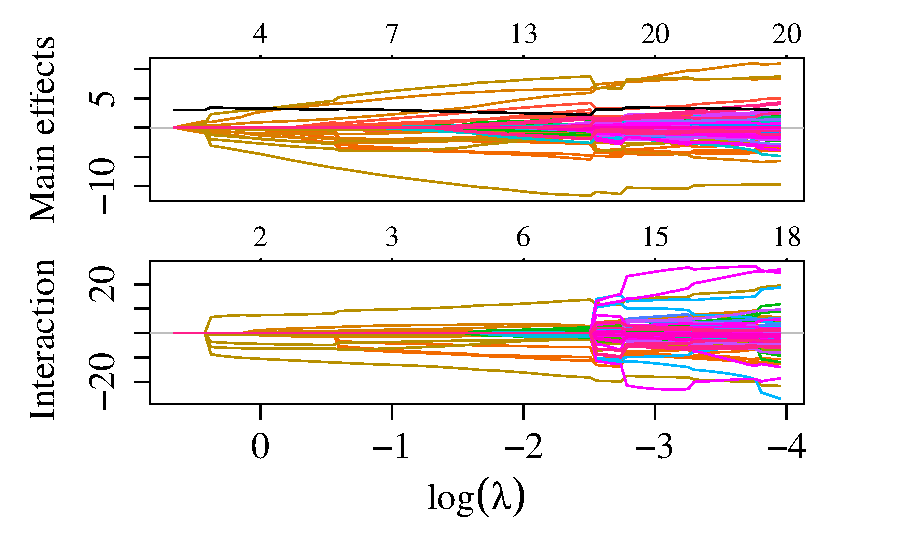
\includegraphics[width=1\linewidth]{figs/sail-pf-path-1} 
				
			}
			
			
			
			\end{knitrout}
			
			
			We see from the plot above that the black line (corresponding to the $X_E$ variable with \texttt{penalty.factor} equal to zero) is always included in the model.   
			
			\subsection{User-Defined Design Matrix} \label{ap:userdesign}
			
			A limitation of the  \texttt{sail} method is that the same basis expansion function $f(\cdot)$ is applied to all columns of the predictor matrix $\mathbf{X}$. Being able to automatically select linear vs. nonlinear components was not a focus of our paper, but is an active area of research for main effects only e.g. \href{https://cran.r-project.org/package=gamsel}{\texttt{gamsel}} and \href{https://github.com/asadharis/HierBasis}{\texttt{HierBasis}}.   
			
			However, if the user has some prior knowledge on possible effect relationships, then they can supply their own design matrix. This can be useful for example, when one has a combination of categorical (e.g. gender, race) and continuous variables, but would only like to apply $f(\cdot)$ on the continuous variables. We provide an example below to illustrate this functionality.  
			
			We use the simulated dataset \texttt{sailsim} provided in our package. We first add a categorical variable \texttt{race} to the data:
			
			\begin{knitrout}\scriptsize
			\definecolor{shadecolor}{rgb}{0.969, 0.969, 0.969}\color{fgcolor}\begin{kframe}
			\begin{alltt}
			\hlkwd{set.seed}\hlstd{(}\hlnum{1234}\hlstd{)}
			\hlkwd{library}\hlstd{(sail)}
			\hlstd{x_df} \hlkwb{<-} \hlkwd{as.data.frame}\hlstd{(sailsim}\hlopt{$}\hlstd{x)}
			\hlstd{x_df}\hlopt{$}\hlstd{race} \hlkwb{<-} \hlkwd{factor}\hlstd{(}\hlkwd{sample}\hlstd{(}\hlnum{1}\hlopt{:}\hlnum{2}\hlstd{,} \hlkwd{nrow}\hlstd{(x_df),} \hlkwc{replace} \hlstd{=} \hlnum{TRUE}\hlstd{))}
			\hlkwd{table}\hlstd{(x_df}\hlopt{$}\hlstd{race)}
		\end{alltt}
		\begin{verbatim}
		## 
		##  1  2 
		## 55 45
		\end{verbatim}
	\end{kframe}
\end{knitrout}

We then use the \texttt{model.matrix} function to create the design matrix. Note that the intercept should not be included, as this is computed internally in the \texttt{sail} function. This is why we add 0 to the formula. Notice also the flexibility we can have by including different basis expansions to each predictor:

\begin{knitrout}\scriptsize
	\definecolor{shadecolor}{rgb}{0.969, 0.969, 0.969}\color{fgcolor}\begin{kframe}
		\begin{alltt}
			\hlkwd{library}\hlstd{(splines)}
			\hlstd{x} \hlkwb{<-} \hlstd{stats}\hlopt{::}\hlkwd{model.matrix}\hlstd{(}\hlopt{~} \hlnum{0} \hlopt{+}  \hlkwd{bs}\hlstd{(X1,} \hlkwc{degree} \hlstd{=} \hlnum{5}\hlstd{)} \hlopt{+} \hlkwd{bs}\hlstd{(X2,} \hlkwc{degree} \hlstd{=} \hlnum{3}\hlstd{)} \hlopt{+} \hlkwd{ns}\hlstd{(X3,} \hlkwc{df} \hlstd{=} \hlnum{8}\hlstd{)} \hlopt{+}
			\hlkwd{bs}\hlstd{(X4,} \hlkwc{degree} \hlstd{=} \hlnum{6}\hlstd{)} \hlopt{+} \hlstd{X5} \hlopt{+} \hlkwd{poly}\hlstd{(X6,}\hlnum{2}\hlstd{)} \hlopt{+} \hlstd{race,} \hlkwc{data} \hlstd{= x_df)}
			\hlkwd{head}\hlstd{(x)}
		\end{alltt}
		\begin{verbatim}
		##   bs(X1, degree = 5)1 bs(X1, degree = 5)2 bs(X1, degree = 5)3
		## 1        0.0001654794         0.003945507        0.0470361237
		## 2        0.2470181057         0.345144379        0.2411253263
		## 3        0.1299195522         0.007832449        0.0002360971
		## 4        0.3808392973         0.121815907        0.0194821217
		## 5        0.1737663057         0.014898419        0.0006386822
		## 6        0.1184145931         0.281407715        0.3343772913
		##   bs(X1, degree = 5)4 bs(X1, degree = 5)5 bs(X2, degree = 3)1
		## 1        2.803692e-01        6.684809e-01           0.3272340
		## 2        8.422768e-02        1.176866e-02           0.3065738
		## 3        3.558391e-06        2.145244e-08           0.1896790
		## 4        1.557896e-03        4.983113e-05           0.4100900
		## 5        1.368987e-05        1.173746e-07           0.3946500
		## 6        1.986587e-01        4.721047e-02           0.3175164
		##   bs(X2, degree = 3)2 bs(X2, degree = 3)3 ns(X3, df = 8)1 ns(X3, df = 8)2
		## 1          0.41274967         0.173537682      0.06566652               0
		## 2          0.04879618         0.002588901      0.00000000               0
		## 3          0.01508834         0.000400076      0.00000000               0
		## 4          0.12345871         0.012389196      0.00000000               0
		## 5          0.35302552         0.105263760      0.00000000               0
		## 6          0.05370432         0.003027827      0.00000000               0
		##   ns(X3, df = 8)3 ns(X3, df = 8)4 ns(X3, df = 8)5 ns(X3, df = 8)6
		## 1     0.000000000    0.000000e+00       0.0000000   -1.589937e-01
		## 2     0.000000000    5.775107e-04       0.3179489    5.395130e-01
		## 3     0.000000000    4.989926e-03       0.4147696    4.830810e-01
		## 4     0.133404268    6.839146e-01       0.1826811    3.022366e-08
		## 5     0.000000000    8.944913e-05       0.2775548    5.564842e-01
		## 6     0.001578195    3.415384e-01       0.6070588    4.566909e-02
		##   ns(X3, df = 8)7 ns(X3, df = 8)8 bs(X4, degree = 6)1 bs(X4, degree = 6)2
		## 1    4.436233e-01   -2.846296e-01        0.1820918880        0.3088147022
		## 2    1.732713e-01   -3.131078e-02        0.0120101010        0.0000608354
		## 3    1.434410e-01   -4.628144e-02        0.0002900763        0.0044075535
		## 4    7.673343e-09   -4.923233e-09        0.2978877432        0.0579746877
		## 5    1.863219e-01   -2.045032e-02        0.0114895681        0.0645689076
		## 6    1.159471e-02   -7.439189e-03        0.0102152807        0.0595722132
		##   bs(X4, degree = 6)3 bs(X4, degree = 6)4 bs(X4, degree = 6)5
		## 1        2.793213e-01        1.421126e-01        3.856204e-02
		## 2        1.643482e-07        2.497444e-10        2.024070e-13
		## 3        3.571755e-02        1.628127e-01        3.958163e-01
		## 4        6.017595e-03        3.513419e-04        1.094046e-05
		## 5        1.935272e-01        3.262743e-01        2.933747e-01
		## 6        1.852831e-01        3.241534e-01        3.024572e-01
		##   bs(X4, degree = 6)6         X5 poly(X6, 2)1 poly(X6, 2)2 race1 race2
		## 1        4.359896e-03 0.51332996  -0.13705545   0.09851639     1     0
		## 2        6.835086e-17 0.02643863   0.18835303   0.22584415     0     1
		## 3        4.009478e-01 0.76746637  -0.15841216   0.16140597     0     1
		## 4        1.419483e-07 0.69077618  -0.03664279  -0.07954100     0     1
		## 5        1.099135e-01 0.27718210   0.13128945   0.05620199     0     1
		## 6        1.175889e-01 0.48384748   0.08486354  -0.03559388     0     1
		\end{verbatim}
	\end{kframe}
\end{knitrout}

One benefit of using \texttt{stats::model.matrix} is that it returns the group membership as an attribute:

\begin{knitrout}\scriptsize
	\definecolor{shadecolor}{rgb}{0.969, 0.969, 0.969}\color{fgcolor}\begin{kframe}
		\begin{alltt}
			\hlkwd{attr}\hlstd{(x,} \hlstr{"assign"}\hlstd{)}
		\end{alltt}
		\begin{verbatim}
		##  [1] 1 1 1 1 1 2 2 2 3 3 3 3 3 3 3 3 4 4 4 4 4 4 5 6 6 7 7
		\end{verbatim}
	\end{kframe}
\end{knitrout}

The group membership must be supplied to the \texttt{sail} function. This information is needed for the group lasso penalty, which will select the whole group as zero or non-zero.

\subsubsection{Fit the \sail ~Model}

We need to set the argument \texttt{expand = FALSE} and provide the group membership. The first element of the group membership corresponds to the first column of \texttt{x}, the second element to the second column of \texttt{x}, and so on. 



We can plot the solution path for both main effects and interactions using the \texttt{plot} method for objects of class \texttt{sail}:

\begin{knitrout}\scriptsize
	\definecolor{shadecolor}{rgb}{0.969, 0.969, 0.969}\color{fgcolor}
	
	{\centering 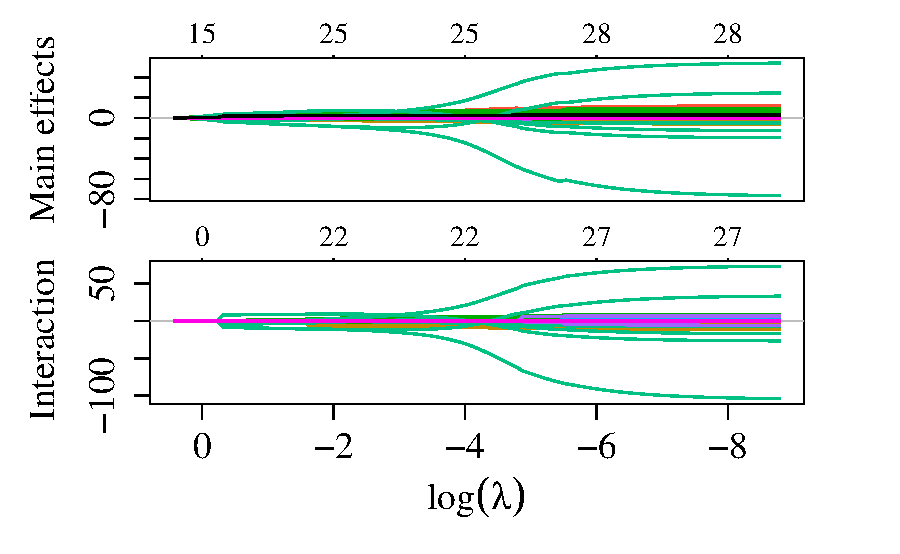
\includegraphics[width=1\linewidth]{figs/sail-expand-false-1} 
		
	}
	
	
	
\end{knitrout}

In this instance, since we provided a user-defined design matrix and `expand = FALSE`, the numbers at the top of the plot represent the total number of non-zero coefficients. 


\subsubsection{Find the Optimal Value for $\lambda$}

We can use cross-validation to find the optimal value of lambda:



We can plot the cross-validated mean squared error as a function of lambda:

\begin{knitrout}\scriptsize
	\definecolor{shadecolor}{rgb}{0.969, 0.969, 0.969}\color{fgcolor}
	
	{\centering 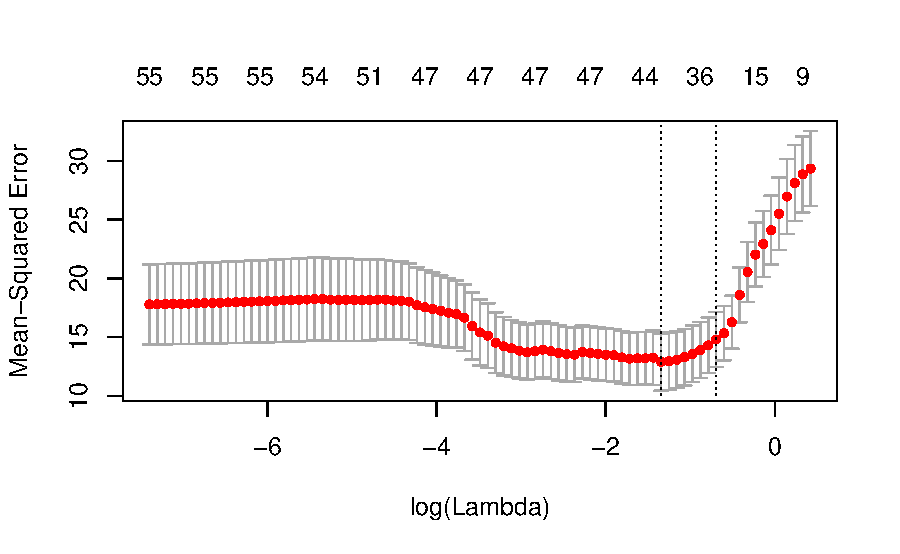
\includegraphics[width=1\linewidth]{figs/sail-plot-cv-design-1} 
		
	}
	
	
	
\end{knitrout}


The estimated non-zero coefficients at \texttt{lambda.1se}:

\begin{knitrout}\scriptsize
	\definecolor{shadecolor}{rgb}{0.969, 0.969, 0.969}\color{fgcolor}\begin{kframe}
		\begin{verbatim}
		##                                  1
		## (Intercept)            5.427451767
		## bs(X1, degree = 5)1   -0.525424522
		## bs(X1, degree = 5)2    0.052358374
		## bs(X1, degree = 5)3    0.271119758
		## bs(X1, degree = 5)4    0.554195548
		## bs(X1, degree = 5)5    1.330393115
		## ns(X3, df = 8)1        2.349455333
		## ns(X3, df = 8)2        2.089923982
		## ns(X3, df = 8)3        0.666828606
		## ns(X3, df = 8)4       -1.200690572
		## ns(X3, df = 8)5       -1.662360501
		## ns(X3, df = 8)6       -1.365480040
		## ns(X3, df = 8)7        0.516186563
		## ns(X3, df = 8)8       -1.215186213
		## bs(X4, degree = 6)1    4.466614577
		## bs(X4, degree = 6)2   -0.252832683
		## bs(X4, degree = 6)3   -4.706674900
		## bs(X4, degree = 6)4   -4.868782936
		## bs(X4, degree = 6)5   -2.105379737
		## bs(X4, degree = 6)6   -0.213392506
		## race1                  0.006726548
		## race2                 -0.006726548
		## E                      1.963105161
		## ns(X3, df = 8)1:E      1.170879214
		## ns(X3, df = 8)2:E      1.041538657
		## ns(X3, df = 8)3:E      0.332322025
		## ns(X3, df = 8)4:E     -0.598378532
		## ns(X3, df = 8)5:E     -0.828457273
		## ns(X3, df = 8)6:E     -0.680503338
		## ns(X3, df = 8)7:E      0.257247758
		## ns(X3, df = 8)8:E     -0.605602609
		## bs(X4, degree = 6)1:E  8.430067510
		## bs(X4, degree = 6)2:E -0.477183905
		## bs(X4, degree = 6)3:E -8.883145495
		## bs(X4, degree = 6)4:E -9.189100187
		## bs(X4, degree = 6)5:E -3.973589620
		## bs(X4, degree = 6)6:E -0.402746465
		\end{verbatim}
	\end{kframe}
\end{knitrout}
